\documentclass[anon]{colt2020} % Anonymized submission
% \documentclass{colt2020} % Include author names

% The following packages will be automatically loaded:
% amsmath, amssymb, natbib, graphicx, url, algorithm2e

\title[Embedding dimension]{Embedding Dimension of Polyhedral Losses}
\usepackage{times}

\usepackage{lmodern}
\usepackage{hyperref}       % hyperlinks  %[implicit=false, bookmarks=false]
\usepackage{booktabs}       % professional-quality tables
\usepackage{amsfonts}       % blackboard math symbols
\usepackage{nicefrac}       % compact symbols for 1/2, etc.
\usepackage{microtype}      % microtypography

\usepackage{mathtools, verbatim}
%\usepackage[thmmarks, thref, amsthm]{ntheorem}
\usepackage{color}
\definecolor{darkblue}{rgb}{0.0,0.0,0.2}
\hypersetup{colorlinks,breaklinks,
	linkcolor=darkblue,urlcolor=darkblue,
	anchorcolor=darkblue,citecolor=darkblue}
\usepackage{wrapfig}
\usepackage{subcaption}
\usepackage[colorinlistoftodos,textsize=tiny]{todonotes} % need xargs for below
%\usepackage{accents}
\usepackage{bbm}
\usepackage{xspace}

%\usetikzlibrary{calc}
\newcommand{\Comments}{1}
\newcommand{\mynote}[2]{\ifnum\Comments=1\textcolor{#1}{#2}\fi}
\newcommand{\mytodo}[2]{\ifnum\Comments=1%
	\todo[linecolor=#1!80!black,backgroundcolor=#1,bordercolor=#1!80!black]{#2}\fi}
\newcommand{\raf}[1]{\mynote{green}{[RF: #1]}}
\newcommand{\raft}[1]{\mytodo{green!20!white}{RF: #1}}
\newcommand{\jessie}[1]{\mynote{purple}{[JF: #1]}}
\newcommand{\jessiet}[1]{\mytodo{purple!20!white}{JF: #1}}
\newcommand{\bo}[1]{\mynote{blue}{[Bo: #1]}}
\newcommand{\botodo}[1]{\mytodo{blue!20!white}{[Bo: #1]}}
\newcommand{\btw}[1]{\mytodo{orange!20!white}{BTW: #1}}
\ifnum\Comments=1               % fix margins for todonotes
\setlength{\marginparwidth}{1in}
\fi


\newcommand{\reals}{\mathbb{R}}
\newcommand{\posreals}{\reals_{>0}}%{\reals_{++}}
\newcommand{\nonnegreals}{\reals_{\geq 0}}%{\reals_{++}}
\newcommand{\dom}{\mathrm{dom}}
\newcommand{\epi}{\text{epi}}
\newcommand{\relint}{\mathrm{relint}}
\newcommand{\prop}[1]{\Gamma[#1]}
\newcommand{\eliccts}{\mathrm{elic}_\mathrm{cts}}
\newcommand{\eliccvx}{\mathrm{elic}_\mathrm{cvx}}
\newcommand{\elicpoly}{\mathrm{elic}_\mathrm{pcvx}}
\newcommand{\elicembed}{\mathrm{elic}_\mathrm{embed}}

\newcommand{\cell}{\mathrm{cell}}

\newcommand{\abstain}[1]{\mathrm{abstain}_{#1}}
\newcommand{\mode}{\mathrm{mode}}

\newcommand{\simplex}{\Delta_\Y}

% alphabetical order, by convention
\newcommand{\C}{\mathcal{C}}
\newcommand{\D}{\mathcal{D}}
\newcommand{\E}{\mathbb{E}}
\newcommand{\F}{\mathcal{F}}
\renewcommand{\H}{\mathcal{H}}
\newcommand{\N}{\mathcal{N}}
\newcommand{\I}{\mathcal{I}}
\newcommand{\R}{\mathcal{R}}
\newcommand{\T}{\mathcal{T}}
\newcommand{\U}{\mathcal{U}}
\newcommand{\V}{\mathcal{V}}
\newcommand{\X}{\mathcal{X}}
\newcommand{\Y}{\mathcal{Y}}
\renewcommand{\P}{\mathcal{P}}

\newcommand{\hinge}{L_{\mathrm{hinge}}}
\newcommand{\ellzo}{\ell_{\text{0-1}}}
\newcommand{\ellabs}[1]{\ell_{#1}}

\newcommand{\Opt}{\mathrm{Opt}}
\newcommand{\risk}[1]{\underline{#1}}
\newcommand{\inprod}[2]{\langle #1, #2 \rangle}%\mathrm{int}(#1)}
\newcommand{\inter}[1]{\mathrm{int}(#1)}%\mathrm{int}(#1)}
%\newcommand{\expectedv}[3]{\overline{#1}(#2,#3)}
\newcommand{\expectedv}[3]{\E_{Y\sim{#3}} {#1}(#2,Y)}
\newcommand{\toto}{\rightrightarrows}
\newcommand{\strip}{\mathrm{strip}}
\newcommand{\trim}{\mathrm{trim}}
\newcommand{\fplc}{finite-piecewise-linear and convex\xspace} %xspace for use in text
\newcommand{\conv}{\mathrm{conv}}
\newcommand{\indopp}{\bar{\mathbbm{1}}}
\newcommand{\ones}{\mathbbm{1}}
\DeclarePairedDelimiter\ceil{\lceil}{\rceil}

\newcommand{\Ind}[1]{\mathbf{1}\{#1\}}

\DeclareMathOperator*{\argmax}{arg\,max}
\DeclareMathOperator*{\argmin}{arg\,min}
\DeclareMathOperator*{\arginf}{arg\,inf}
\DeclareMathOperator*{\sgn}{sgn}

%\newtheorem{theorem}{Theorem}
%\newtheorem{lemma}{Lemma}
%\newtheorem{proposition}{Proposition}
%\newtheorem{definition}{Definition}
%\newtheorem{corollary}{Corollary}
%\newtheorem{conjecture}{Conjecture}
\newtheorem{observation}{Observation}
\newtheorem{condition}{Condition}
\newtheorem{claim}{Claim}
% Use \Name{Author Name} to specify the name.
% If the surname contains spaces, enclose the surname
% in braces, e.g. \Name{John {Smith Jones}} similarly
% if the name has a "von" part, e.g \Name{Jane {de Winter}}.
% If the first letter in the forenames is a diacritic
% enclose the diacritic in braces, e.g. \Name{{\'E}louise Smith}

% Two authors with the same address
% \coltauthor{\Name{Author Name1} \Email{abc@sample.com}\and
%  \Name{Author Name2} \Email{xyz@sample.com}\\
%  \addr Address}

% Three or more authors with the same address:
 \coltauthor{\Name{Jessie Finocchiaro} \Email{jefi8453@colorado.edu}\\
  \Name{Rafael Frongillo} \Email{raf@colorado.edu}\\
  \Name{Bo Waggoner} \Email{bwag@colorado.edu}\\
  \addr CU Boulder}

% Authors with different addresses:
%\coltauthor{%
% \Name{Jessie Finocchiaro} \Email{jefi8453@colorado.edu}\\
% \addr CU Boulder
% \AND
% \Name{Rafael Frongillo} \Email{Raf@colorado.edu}\\
% \addr CU Boulder
% \AND
% \Name{Bo Waggoner} \Email{bwag@colorado.edu}\\
% \addr CU Boulder%
%}

\begin{document}

\maketitle

\begin{abstract}%
  A common technique in supervised learning with discrete losses, such as $0-1$ loss, is to optimize a convex surrogate loss over $\reals^d$, calibrated with respect to the original loss.
  In particular, recent work has investigated embedding the original predictions (e.g. labels) as points in $\reals^d$.
  %Recent work has proposed the notion of designing calibrated surrogate losses for classification-like problems through the lens of \emph{embedding} the original problem into $\reals^d$ and optimizing a polyhedral loss that is calibrated with respect to the original loss.
  In this work, we study the notion of \emph{embedding dimension} for given discrete losses.
  We characterize when a given discrete loss can be embedded into the real line, as well as when a higher-dimensional input to the surrogate loss is required.
  Moreover, we give a quadratic feasibility program that yields lower bounds on the embedding dimension of a given discrete loss.
\end{abstract}

\begin{keywords}%
  Calibrated surrogates, convex surrogates, proper scoring rules%
\end{keywords}


%%%%%%%%%%%%%%%%%%%%%%%%%%%%%%%%%%%%%%%%%%%%%%%%%%%%%%%%%%%%%%%%
\section{Introduction}
In supervised machine learning, the dominant paradigm is to measure performance of a model using some loss function $\ell($prediction, observation$)$.
In particular, this paper studies \emph{discrete} losses, in which the predictions lie in a finite set.
These are popular for many categorical tasks such as classification, ranking, top-$k$, set inclusion, and other structured prediction tasks.
%Models are trained using some variant of empirical risk minimization, i.e. minimization of loss on a training data set.
%For many categorical tasks (e.g. classification, ranking, top-$k$, set inclusion), one can often use intuition to design a discrete loss $\ell$ that models the question one wants to answer about one's data.
%For example, $0-1$ loss $\ell(r)_y = \Ind{r \neq y}$ gives punishment $1$ for a misprediction and $0$ for a correct prediction, and is used for classification problems over possibly large finite category sets.

However, the optimization of discrete losses over a dataset (i.e. empirical risk minimization) is typically computationally hard.
One therefore generally resorts to optimizing a computationally-nice \emph{surrogate loss} $L$.
The key requirement is \emph{calibration}, namely that optimizing surrogate loss allows one to recover the discrete prediction that optimizes the original $\ell$-loss.
Calibrated surrogate losses yields desirable statistical guarantees such as the existence of excess risk bounds given by consistency~\citep{tewari2007consistency}.
%In the finite outcome setting, we know that calibration implies consistency, so we study the design of calibrated, convex losses-- specifically polyhedral (piecewise linear and convex) losses.

The question therefore becomes: Given a discrete loss $\ell$, how do we design such calibrated surrogates $L$? 
The class of surrogates studied in this paper are \emph{polyhedral}, meaning piece-wise linear convex functions over prediction space $\reals^d$.
\cite{finocchiaro2019embedding} show that polyhedral surrogates are equivalent to the following recipe: \emph{embedding} the discrete loss $\ell$ into $\reals^d$ by letting each discrete prediction $r$ correspond to some point $\varphi(r) \in \reals^d$, which optimizes $L$-loss if and only if $r$ optimizes $\ell$-loss.
\cite{finocchiaro2019embedding} show that every discrete loss $\ell$ can be embedded into \emph{some} dimension $d$.
But in the worst case $d=n-1$ where $n$ is the number of possible observations $y$, e.g. a number of classification categories.

%\emph{embedding losses} in order to construct polyhedral, calibrated surrogate losses for a given discrete loss.
%Their work constructively shows that every discrete loss is embeddable, but it is unclear how efficient an embedding can get.
In this work, we define and investigate the \emph{embedding dimension} of discrete losses.
A loss $\ell$ is $d$-embeddable if it can be embedded in $\reals^d$, equivalently, has some calibrated polyhedral surrogate $L$ over $\reals^d$.
Given $\ell$, it is desirable for computational and statistical reasons to construct a surrogate in as few dimensions as possible; it is also interesting to prove lower bounds, i.e. that no calibrated surrogate exists unless $d$ is large enough.

\paragraph{Contributions.}
In particular, $1$-embeddings have the simplest possible convex surrogate space, the real line.
In Section~\ref{sec:1d}, we characterize $1$-embeddability of a discrete loss $\ell$ via a variety of conceptual and testable conditions.
We give an efficient algorithm that, given the loss matrix of $\ell$, either proves that $\ell$ is not $1$-embeddable, or else constructs a calibrated $1$-dimensional polyhedral surrogate.
We also show that, perhaps surprisingly, for $d=1$, if \emph{any} convex calibrated surrogate exists, then in particular a polyhedral one does.
We conjecture that this continues to hold in higher dimensions.\bo{Formalize conjecture later?}
In other words, we conjecture that embedding dimension is actually always equal to the more permissive \emph{convex calibration dimension} of \cite{ramaswamy2016convex}.

In Section~\ref{sec:d-dim}, we observe a general characterization for $d \geq 2$, presenting conditions called optimality and monotonicity that are necessary and sufficient for $d$-embeddability.
A particular contribution is to isolate and investigate the optimality condition, which reduces to a finite set of conditions on the halfspace and vertex representations of a set of polytopes related to $\ell$ and $L$.
This allows us to construct a Quadratic Feasibility Program (Definition~\ref{def:qfp}) that has a solution if and only if the optimality condition can be satisfied.
In addition to providing a possible avenue toward automating the search for calibrated surrogate losses, this feasibility program yields new techniques for lower bounds on the embedding dimension of a given discrete loss.

In Section~\ref{sec:examples}, we apply our characterizations to show new lower bounds on the embedding dimension for a problem, classification with an abstain option, whose convex calibration dimension has been well-studied (\cite{ramaswamy2016convex, ramaswamy2018consistent}).
%These results suggest that \emph{if} the convex calibration dimension of the same problems were lower than the embedding dimension, constructing a calibrated surrogate for such problems would require a new approach than previous works have taken.
In particular we apply both our $1$-dimension characterization and higher-dimensional quadratic program to obtain previously-unknown lower bounds.

\subsection{Related work}
\cite{bartlett2006convexity} study when a convex, calibrated surrogate exists for a given discrete loss, and in a finite-outcome setting,~\cite{tewari2007consistency} show that calibration (Definition~\ref{def:calibration}) is necessary and sufficient for consistency.
%, meaning that there is a link mapping surrogate reports to discrete reports so that converging to the optimal prediction in the surrogate space implies the linked surrogate prediction converges to the optimal prediction for the original loss.

Several works have investigated the problem of reducing the dimensionality of a surrogate loss.
\cite{frongillo2015elicitation} propose \emph{elicitation complexity}, which roughly captures the minimum dimension $d$ of any surrogate loss $L$ (not necessarily convex or calibrated) for a given loss $\ell$ (not necessarily discrete).
In the more specific case of convex calibrated surrogates for discrete losses,~\cite{ramaswamy2016convex} propose the notion of \emph{convex calibration dimension}, which is the minimum dimension input to a convex surrogate loss that is calibrated with respect to a given discrete loss.
The difference in this paper is that our definition of embedding dimension requires the surrogate loss to additionally be polyhedral.
\cite{ramaswamy2016convex} present a condition for obtaining lower bounds on convex calibration dimension for any discrete loss, \emph{feasible subspace dimension}.
However, there are important examples, such as the $\ellabs{\alpha}$ loss in Equation~\eqref{eq:abstain}, for which feasible subspace dimension gives only trivial bounds.
A contribution of this work is to provide the first nontrivial lower bounds for this loss (see also discussion in Section \ref{sec:conclusion}).

\cite{ramaswamy2018consistent} present upper bounds on the convex calibration of $\abstain{\alpha}$ loss of $\ceil{\log_2(n)}$, but their characterization of lower bounds leave the tightness of these bounds as an open question.
These upper bounds are, however, much tighter than the previous upper bounds of $(n-1)$ given by the different surrogates presented by~\cite{crammer2001algorithmic} and~\cite{rifkin2004defense}, and it is unclear what characteristics of the abstain loss allow us to exponentially reduce dimension of the input.

%In this work, we study \emph{embedding dimension}, which is the minimum dimension of input to a polyhedral surrogate that is calibrated with respect to the given discrete loss.
%Moreover, we use this tool to characterize \emph{how} embeddable a given discrete loss is, showing necessary conditions for embedding a given loss into $d$ dimensions.
In order to concisely discuss embedding dimension, we appeal to notation and terminology from the field of property elicitation (\cite{frongillo2015vector-valued, gneiting2007strictly, lambert2009eliciting, osband1985information-eliciting, savage1971elicitation}), relating it to the language of calibrated surrogates as needed.

%%%%%%%%%%%%%%%%%%%%%%%%%%%%%%%%%%%%%%%%%%%%%%%%%%%%%%%%%%%%%%%%
\section{Setting}

\paragraph{Discrete losses and (polyhedral) surrogates.}

The base object of study is a \emph{discrete loss function} $\ell: \R \to \nonnegreals^{\Y}$ where $\R$ and $\Y$ are finite sets.
Here $\ell(r)_y$ is the loss of prediction $r \in \R$ (the report space) on $y \in \Y$ (the observation or label space).
For simplicity we let $\Y = [n]$ throughout (where $[n] = \{1,\ldots,n\}$).
The set of probability distributions on $\Y$ is denoted $\simplex\subseteq\nonnegreals^{\Y}$, represented as vectors of probabilities.
We write $p_y$ \bo{check/decide}\jessie{Fine with this, and I think it's consistently in the paper like this already} for the probability of outcome $y \in \Y$ drawn from $p \in \simplex$.
As is assumed by~\cite{finocchiaro2019embedding}, we assume the given discrete loss is \emph{non-redundant}, meaning every report $r$ uniquely minimizes expected loss for some distribution $p\in\simplex$.

We similarly denote surrogate losses in dimension $d$ by $L:\reals^d\to\nonnegreals^{\Y}$, with predictions typically written $u\in\reals^d$.
The expected losses when $Y \sim p$ can be written $\inprod{p}{\ell(r)}$ and $\inprod{p}{L(u)}$.
For example, 0-1 loss on two labels is a discrete loss with $\R = \Y = \{-1,1\}$
given by $\ellzo(r)_y = \Ind{r \neq y}$.
Two important surrogates for $\ellzo$ are hinge loss $\hinge(u)_y = \max\{ 0 ~,~ 1-yu \}$ and logistic loss $L(u)_y = \log(1+\exp(-yu))$ for $u\in\reals$.

Most of the surrogates $L$ we consider will be \emph{polyhedral}, meaning piecewise linear and convex; we therefore briefly recall the relevant definitions.
In $\reals^d$, a \emph{polyhedral set} or \emph{polyhedron} is the intersection of a finite number of closed halfspaces.
A \emph{polytope} is a bounded polyhedral set.
A convex function $f:\reals^d\to\reals$ is \emph{polyhedral} if its epigraph is polyhedral, or equivalently, if it can be written as a pointwise maximum of a finite set of affine functions~\citep{rockafellar1997convex}.
%
\begin{definition}[Polyhedral loss]
	A loss $L: \reals^d \to \nonnegreals^{\Y}$ is \emph{polyhedral} if $L(u)_y$ is a polyhedral (piecewise linear convex) function of $u$ for each $y\in\Y$.
\end{definition}
%
For example, hinge loss is polyhedral, whereas logistic loss is not.

\paragraph{Properties of distributions.}
In order to study calibration of surrogates (Definition~\ref{def:calibration} below), it is useful to formalize the following functions that describe the reports that minimize expected $\ell$-loss and $L$-loss under $p$.
%% Bo: since we use \gamma and \R for \ell, and we use \Gamma and \reals^d for L,
%% I figured generic properties could use notation g and R for f
\begin{definition}[(Finite) property, level set, elicited]
  A \emph{property} is a function $g: \simplex \to 2^{R}$ for some set $R$ where $g(p) \neq \emptyset$ for all $p$.
  It is \emph{finite} if $|R| < \infty$.
  The \emph{level set} of $r \in R$ is the set $g_r = \{p \in \simplex : r \in g(p)\}$.
  A loss function $f: R \to \nonnegreals^{\Y}$ \emph{elicits} $g$ if $g(p) = \argmin_{r \in R} \inprod{p}{f(r)}$.
  We assume all properties are non-redundant, i.e. each $g_r$ contains a distribution $p$ not in any other $g_{r'}$.\jessiet{$R$ or $\R$?}
\end{definition}
For example, $0-1$ loss elicits the mode, which is formalized as a property on report space $R = \Y$ via $g(p) = \argmax_{y \in \Y} p_y$.
Notice in this example $g(p)$ is a singleton set when the mode of $p$ is unique and e.g. is $\Y$ when $p$ is uniform.
%Another example of a finite property is ranking, in which $\R$ is the set of permutations of $\Y$, and $g(p)$ consists of all permutations that order $\Y$ from most to least probable (i.e. ties must be broken in all possible ways).
In this paper we write $\gamma$ for the property elicited by $\ell$ with report space $\R$; and we use $\Gamma$ for the property elicited by $L$ with report space $\reals^d$.

\paragraph{Embeddings.}
%We specifically study polyhedral functions in part because they have high-dimensional subgradient sets at points of nondifferentiability, which will be of interest to us later.
Polyhedral losses are motivated partly because they correspond to a natural surrogate construction technique: embedding the discrete predictions $\R$ as points in $\reals^d$ and linearly interpolating between embedded reports.
The key condition required on the embedding and surrogate loss $L$ is that a discrete prediction $r \in \R$ should minimize expected $\ell$-loss if and only if its embedding point minimizes expected $L$-loss.
%
\begin{definition}[Embedding of a loss]
  A loss $L: \reals^d \to \nonnegreals^{\Y}$ \emph{embeds} a loss $\ell: \R \to \nonnegreals^{\Y}$ \emph{in dimension $d$} with \emph{embedding function $\varphi: \R \to \reals^d$} if: (i) $\varphi$ is injective; (ii) for all $r \in \R$, $\ell(r) = L(\varphi(r))$; and (iii) for all $r \in \R$, $\gamma_r = \Gamma_{\varphi(r)}$.
  We simply say $L$ \emph{embeds} $\ell$ if some such $\varphi$ exists.
\end{definition}
%
Note that embedding does not immediately imply a key desirable property, consistency, which is equivalent to calibration in finite-outcome settings.
Informally, calibration means that if one minimizes the expected surrogate loss arbitrarily well over $\reals^d$, then applies the link function to obtain a discrete prediction $r$, then $r$ exactly minimizes $\ell$-loss.
\begin{definition}[Calibrated surrogate]\label{def:calibration}
  A surrogate loss $L: \reals^d \to \nonnegreals^{\Y}$ and \emph{link function} $\psi: \reals^d \to \R$ are \emph{calibrated} for a loss $\ell: \R \to \nonnegreals^{\Y}$ if for all $p \in \simplex$,
    \[ \inf_{u \in \reals^d ~:~ \psi(u) \not\in \gamma(p)} \inprod{p}{L(u)}  > \inf_{u \in \reals^d} \inprod{p}{L(u)}  .\]
  We simply say $L$ can be \emph{calibrated} to $\ell$ if such a link function exists.
\end{definition}
As we alluded to above, calibration is not actually the trait we desire of a surrogate; rather, we seek consistency.
\cite{tewari2007consistency} show that, in a finite-outcome setting, the presence of calibration and consistency are equivalent conditions.
By consistency, we mean the standard notion where the expected loss over $\X \times \Y$ for a sequence of hypotheses $h_m$ converging to the optimal expected surrogate loss implies the expected discrete loss over the linked hypotheses $\psi \circ h_m$ converges to the optimal discrete loss.
The equivalence of these conditions allows us to focus on calibration, so we can abstract away the input space $\X$ and simply focus on probability distributions over the outcomes $\Y$.

%\jessie{Not a smooth transition here...} \bo{I think it's ok...}
Polyhedral surrogates are motivated by the following results.
\begin{theorem}[\cite{finocchiaro2019embedding}] \label{thm:embed-iff-poly}
  If a discrete loss $\ell$ is embedded by some surrogate $L$, then (1) $L$ must be a polyhedral loss; and (2) there exists a link function calibrating $L$ to $\ell$.
\end{theorem}
In other words, polyhedral surrogates are equivalent to embeddings of discrete losses $\ell$ in $\reals^d$; and they come with a guarantee of calibration.
This raises the question studied in this paper: in what dimension $d$ does such a surrogate exist?

\subsection{Embedding dimension}

In this paper, we study the following quantity.
\begin{definition}[Embedding dimension]
  We say a discrete loss $\ell: \R \to \nonnegreals^{\Y}$ is \emph{$d$-embeddable} if it can be embedded into $d$ dimensions, i.e. if there exists a calibrated polyhedral surrogate $L: \reals^d \to \nonnegreals^{\Y}$.
  The \emph{embedding dimension} of $\ell$ is the smallest $d$ such that $\ell$ is $d$-embeddable.
\end{definition}

A number of things are already known about embedding dimension.
Many surrogates in the literature provide upper bounds; we highlight in particular the \emph{abstain loss} given by \cite{ramaswamy2018consistent} and seen in Equation~\eqref{eq:abstain}, in which one wants to predict the most likely outcome \emph{only if} confident in the outcome, and otherwise abstain.

\begin{equation}\label{eq:abstain}
\ellabs{\alpha}(r)_y = \begin{cases}
0 & r = y\\
\alpha & r = \bot\\
1 & r \not \in \{y, \bot\}
\end{cases}
\end{equation}
Here $\R = \Y \cup \{\bot\}$.
For $\alpha=1/2$, \cite{ramaswamy2018consistent} give an elegant embedding of this loss on $n$ outcomes into $d = \lceil \log_2 (n) \rceil$ dimensions, where each $y \in \Y$ is embedded at a corner of the Boolean hypercube $\{-1,1\}^d$ while $\bot$ is embedded at the origin.

In general (e.g. \cite{finocchiaro2019embedding}), a known convex-conjugate construction generically embeds any discrete loss on $\Y = [n]$ into $d = n-1$ dimensions, giving a flat upper bound of $n-1$ on embedding dimension.
Lower bounds exist but are rare.
A lower bound on the dimensionality of \emph{any} calibrated convex surrogate $L$ implies in particular a lower bound on polyhedral surrogates.
\cite{ramaswamy2016convex} give such a lower bound via the technique of \emph{feasible subspace dimension}, which is able to e.g. prove that embedding $0-1$ loss on $n$ labels requires dimension $n-1$.
However, this technique gives only the trivial $d \geq 1$ for the abstain family of losses above when $\alpha \leq 1/2$ because of their geometric structure.
We discuss further in Section \ref{sec:conclusion}.


%%%%%%%%%%%%%%%%%%%%%%%%%%%%%%%%%%%%%%%%%%%%%%%%%%%%%%%%%%%%%%%%
\section{One-dimensional embeddings}
\label{sec:1d}

In this section, we completely characterize when a discrete loss $\ell$ can be embedded into the real line, i.e., when $\ell$ is 1-embeddable.
Our first characterization is expressed in terms of the property $\gamma$ that $\ell$ elicits, stating that $\ell$ is 1-embeddable if and only if $\gamma$ is \emph{orderable}, meaning the adjacency graph of its level sets is a path.
For example, this characterization will immediately imply that embedding the abstain losses on $n \geq 3$ outcomes requires $d \geq 2$ dimensions (\S~\ref{sec:examples}).
While determining these adjacencies can be straightforward when $\ell$ has known symmetries, we also give a more constructive algorithm for testing $1$-embeddability and constructing a $1$-dimensional polyhedral surrogate.
Finally, we show that the existence of any $1$-dimensional convex calibrated implies $1$-embeddability, showing that embeddings are without loss of generality in dimension 1.
After presenting and discussing this sequence of results, we observe that they can be collected as a set of six conditions on $\ell$ that are all pairwise equivalent, and in particular, are equivalent to $1$-embeddability.

\subsection{General characterization via property elicitation}

We begin with conditions on the property elicited by a discrete loss.
The following condition of~\citet[Theorem 3]{lambert2018elicitation}, that a finite property is \emph{orderable}, states that any two level sets intersect in a hyperplane, or not at all.
\begin{definition}[Orderable]\label{def:orderable-hyperplane}
	A finite property $\gamma:\simplex \to 2^\R$ is \emph{orderable} if there is an enumeration of $\R = \{r_1, \ldots, r_{|\R|}\}$ such that for all $i \leq |\R| - 1$, we have $\gamma_{r_i} \cap \gamma_{r_{i+1}}$ is a hyperplane intersected with $\simplex$.
\end{definition}

In fact, we show that orderability characterizes $1$-embeddability.
The proof involves several intermediate results which we state later in this section; see \S~\ref{sec:1d-proof-discuss} for more details. 
\begin{theorem} \label{thm:orderable-iff-1d}
  A discrete loss $\ell$ is $1$-embeddable if and only if the property it elicits is orderable.
\end{theorem}

We next give an equivalent condition to orderability which may be more intuitive: the adjacency graph of the level sets of $\gamma$, formed by connecting reports if their level sets intersect, must be a path.
This graph can be easily established for discrete losses with known symmetries or other facts, such as abstain, the mode, or ranking losses.

\begin{definition}[Intersection graph]\label{def:intersection-graph}
  Given a discrete loss $\ell$ and associated finite property $\gamma: \simplex \toto 2^{\R}$ elicited by $\ell$, the \emph{intersection graph} has vertices $\R$ with an edge $(r,r')$ if $\gamma_r \cap \gamma_{r'} \cap \relint(\simplex) \neq \emptyset$, where $\relint(\simplex)$ is the relative interior of $\simplex$.
  %(distributions with full support).
\end{definition}
\begin{proposition} \label{prop:orderable-iff-path}
  A finite property $\gamma$ is \emph{orderable} if and only if its intersection graph is a path, i.e. a connected graph where every vertex has either one or two neighbors.
\end{proposition}
\begin{proof}
  $(\implies)$
  The intersection graph is constructed by adding an edge for each halfspace, which connects only two nodes.
  If three level sets intersected on $\relint(\simplex)$, then the level boundary for any two would not be a halfspace (this follows because the level sets form a power diagram, e.g. \bo{cite}).
  This yields a path for the intersection graph.
  

  $(\impliedby)$
  \bo{This one needs a bit of work.}
  If the intersection graph forms a path, then each level set has at most two neighbors.
  The level sets are convex polytopes, as they form a power diagram\dots.
  
  As each path has a source, take the corresponding report to be $r_1$, and proceed in order through the path to enumerate the ordering.
  As the property is well-defined on the simplex, the boundaries of the level sets cannot intersect on $\relint(\simplex)$ without adding an edge.
  Combining this fact with the fact that level sets of finite elicitable properties are convex polytopes (and therefore defined as the intersection of a finite number of halfspaces), the level set boundaries must be hyperplanes intersected with $\simplex$. 
\end{proof}

Combining Proposition~\ref{prop:orderable-iff-path} and Theorem~\ref{thm:orderable-iff-1d}, we see that in order for $\ell$ to be embedded onto the real line, it is necessary and sufficient for the intersection graph of the property $\gamma$ to be a path.
We give an example of a direct application in Section \ref{sec:examples}.
By visualizing the level sets of $\gamma$ as a power diagram (generalization of Voronoi diagram) in the simplex~\cite{lambert2009eliciting}, we can also use Proposition~\ref{prop:orderable-iff-path} to perform a visual test for orderability, and thus 1-embeddability (Figures~\ref{fig:intersection-graph-ex} and~\ref{fig:abstain-alpha-half}).

\begin{figure}
	\begin{minipage}{0.48\linewidth}
	\centering
	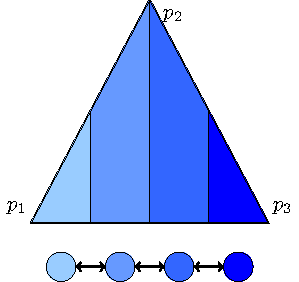
\includegraphics[width = 0.8\linewidth]{tikz/intersection-graph.pdf}
	\caption{The simplex on $3$ outcomes, with the level sets and intersection graph for the [truncated] expected value property on outcomes $\Y = \{1,2,3\}$.}
	\label{fig:intersection-graph-ex}
	\end{minipage}
\hfill
	\begin{minipage}{0.48\linewidth}
	\centering
	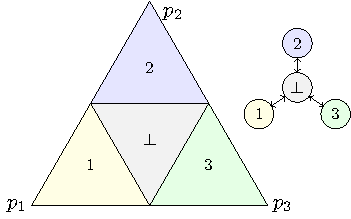
\includegraphics[width = 0.9\linewidth]{tikz/abstain-alpha-half.pdf}
	\caption{Level sets and intersection graph for the $\abstain{1/2}$ property on $\Y = \{1,2,3\}$.}
	\label{fig:abstain-alpha-half}
\end{minipage}
\end{figure}

\subsection{Constructing a surrogate}
While Theorem~\ref{thm:orderable-iff-1d} and Proposition~\ref{prop:orderable-iff-path} are quite useful for discrete losses with known symmetries, they do not immediately provide an algorithm to test $1$-embeddability of an arbitrary discrete loss $\ell$, nor to construct the convex loss $L$ which embeds it.
We now turn to a more algorithmic test, which will actually build a real-valued polyhedral calibrated surrogate in the event that $\ell$ is $1$-embeddable.

%\begin{algorithm}
%  \SetAlgoLined
%  \KwInput{discrete loss $\ell: \R \to \nonnegreals^{\Y}$}
%  Let $v_i(y) = \ell(r_i)$
%\end{algorithm}

\begin{theorem} \label{thm:construct-1d-loss}
  Let $\ell: \R \to \nonnegreals^{\Y}$ be a discrete loss.
  Then $\ell$ is $1$-embeddable if and only if there is an ordering $\R = \{r_1,\ldots,r_k\}$ of the reports such that the following two conditions hold, where $v(i)_y := \ell(r_i)_y - \ell(r_{i-1})_y$:
  \begin{enumerate}
  \item For all $y\in\Y$, the sequence $\sgn(v(i)_y)$ is monotone in
    $i\in\{1,\ldots,k-1\}$,
  \item For all $i\in\{2,\ldots,k-1\}$
    \begin{align*}
      \lambda^-(i) &= \min \left\{\frac{v(i)_y}{v({i+1})_y} : y\in\Y, v(i)_y, v({i+1})_y < 0\right\}
      \\
      \lambda^+(i) &= \max \left\{\frac{v(i)_y}{v({i+1})_y} : y\in\Y, v(i)_y, v({i+1})_y > 0\right\}~,
    \end{align*}
    we have $\lambda^-(i) \geq \lambda^+(i)$.
    (We adopt the convention $\max\emptyset = -\infty$, $\min\emptyset = +\infty$.)
  \end{enumerate}

  Moreover, when these conditions hold, the loss $L:\reals\to\reals^\Y$ embeds $\ell$ with $\varphi:\R\to\reals$,
  where
  \begin{align*}
    \varphi(r_i) &= \sum_{j=1}^{i-1} 1/\Lambda_j~, \quad \text{(where $\varphi(r_1)=0$)}
    \\
    L(u) &= \begin{cases}
      \ell(r_1) - u K \ones & u \leq \varphi(r_1) = 0 \\
      \ell(r_i) + \Lambda_i \cdot (u - \varphi(r_i)) \cdot  (\ell(r_{i+1})-\ell(r_i)) & u \in [\varphi(r_i),\varphi(r_{i+1})] \\
      \ell(r_k) + \Lambda_{k-1} \cdot (u - \varphi(r_k))\cdot K \ones & u \geq \varphi(r_k)
    \end{cases}~,
  \end{align*}
  \jessiet{In the cases: what if $\varphi(r_1) < 0$?}\raft{I set $\varphi(r_1)=0$; updated to something hopefully clearer}
  where $\lambda(i) = \min(\lambda^+(i),\max(\lambda^-(i),1))$, $\Lambda_i := \prod_{j=2}^i \lambda(j)$, $\Lambda_1=1$, and $K = \max_{i\in\{2,\ldots,k\},y\in\Y} |v(i)_y|$.
\end{theorem}
As intuition for the proof, note that the conditions of the theorem ensure the existence of a positive multiplier $\lambda(i)$ making $v(i) \leq \lambda(i) v(i+1)$ hold coordinate-wise; our choice of $\lambda(i)$ is but one option.
The construction of $L$ sets the left and right derivatives at an embedding point $\varphi(r_i)$ to be positive multiples of $v(i)$ and $v(i+1)$, respectively, using this inequality to maintain monotonicity, and hence convexity of $L$.
The vectors $v(i),v(i+1)$ are chosen precisely to give the correct optimality conditions, so that for a given distribution, $r_i$ is optimal for $\ell$ if and only if $\varphi(r_i)$ is optimal for $L$.
The reverse direction, showing that these conditions are necessary for $1$-embeddability, is much more involved (\S~\ref{sec:1d-proof-discuss}).


Note that a calibrated surrogate should also specify a link function $\psi: \reals^d \to \R$.
As our surrogate is an embedding, Theorem \ref{thm:embed-iff-poly} guarantees the existence of a link achieving calibration.
We can also easily construct one in the case of $d=1$, by taking the midpoints between the embedding points as cutoffs: $\psi(u) = \argmin_{r \in \R} |u - \varphi(r)|$, breaking ties arbitrarily.

\subsection{Proof techniques and general convex surrogates}
\label{sec:1d-proof-discuss}

\raf{*much* more to say here...}

We collect the above results, and add one more, in the following summary theorem.
\begin{theorem} \label{thm:1d-tfae}
  Let $\ell: \R \to \nonnegreals^{\Y}$ be a discrete loss eliciting a finite property $\gamma$.
  The following are equivalent: (1) $\gamma$ is orderable; (2) the intersection graph of $\gamma$ is a path; (3) the two conditions of Theorem \ref{thm:construct-1d-loss} are satisfied; (4) $\ell$ is $1$-embeddable; (5) $\ell$ has some polyhedral calibrated surrogate loss $L: \reals \to \nonnegreals^{\Y}$; (6) $\ell$ has some convex calibrated surrogate loss $L: \reals \to \nonnegreals^{\Y}$.
\end{theorem}

We summarize the proof ideas here.
(1) $\iff$ (2) was shown in Proposition \ref{prop:orderable-iff-path}.
(4) $\iff$ (5) was shown in \cite{finocchiaro2019embedding}, which we summarized in Theorem \ref{thm:embed-iff-poly}.
We therefore prove (1) $\implies$ (3) $\implies$ (4) $\implies$ (6) $\implies$ (1).
\bo{What else to say?}


%%%%%%%%%%%%%%%%%%%%%%%%%%%%%%%%%%%%%%%%%%%%%%%%%%%%%%%%%%%%%%%%
\section{Higher dimensions}\label{sec:d-dim}
Our newfound understanding of the 1-dimensional embedding characterization leads us to realize that a large class of properties are not $1$-embeddable.
\cite{finocchiaro2019embedding} have shown a trivial upper bound that every property is $(n-1)$-embeddable\jessie{already mentioned earlier}, but it is an open question as to how tight we can get the bounds on embedding dimension.
Reducing embedding dimension significantly below $(n-1)$ can help provide a computational speedup in the optimization problem, which is a function of the surrogate loss dimension.
This is especially important as the number of possible outcomes $n$ grows large.

Below, we generalize our characterization to $d$-embeddability for $d \geq 2$.
Having a finite number of embedding points and restricting to polyhedral functions allows us to study the subgradient sets of the loss at embedding points, which we formalize in Section~\ref{subsec:sub-sets}.
Using a general theory of polytopes, we can then present our general $d$-dimensional characterization in terms of optimality and monotonicity conditions.
In Section~\ref{subsec:opt-conditions}, we present a quadratic feasibility program in order to understand necessary conditions for $d$-embeddability by satisfying optimality conditions, yielding new lower bounds for embedding dimension in Corollary~\ref{cor:d-embeddable-char}.

\subsection{Setup: subgradient sets at embedding points.}\label{subsec:sub-sets}
%Recall that we have a loss function $\ell: \R \to \reals^{\Y}_{\geq 0}$, and for any prediction $r \in \R$ of the algorithm, we write $\gamma_r = \{ p : \inprod{p}{\ell(r)} \leq \inprod{p}{\ell(r')} (\forall r')\}$.
%We are interested in potential polyhedral surrogates $L: \reals^d \to \reals^{\Y}_{\geq 0}$.
%These are associated with embedding points, where $u_r \in \reals^d$ is linked back to the discrete prediction $r$.

Recall that if $\ell: \R \to \nonnegreals^{\Y}$ is embedded by $L: \reals^d \to \nonnegreals^{\Y}$, then each $r \in \R$ is embedded at some point $u_r \in \reals^d$.
In particular, $u_r$ must minimize $\inprod{p}{L(u)}$ if and only if $r$ minimizes $\inprod{p}{\ell(r')}$.

The key to our approach is to study as first-class objects the sets of all subgradients\footnote{Recall that a subgradient of e.g. the convex function $L(\cdot)_y: \reals^d \to \reals$ at a point $u$ is a vector $v \in \reals^d$ such that $L(u')_y \geq L(u)_y + \inprod{v}{u'-u}$ for all $u'$.} of $L$ at these embedding points.
To settle the question of whether a consistent surrogate exists in $d$ dimensions, it surprisingly turns out to be necessary and sufficient to consider conditions on these sets alone.
In particular, we use heavily that a convex function is minimized at a point if and only if the origin $\vec{0}$ is in its subgradient set at that point.

Therefore, we abstract to consider collections of sets $T^r_y$, which aspire to be the subgradient sets of a calibrated polyhedral surrogate $L(\cdot)_y$ at $u_r$.
Throughout, we fix $r$ and remove it from the subscript for ease of exposition.
Note that if $L(\cdot)_y$ is a polyhedral function on $\reals^d$, then all of its subgradient sets are (bounded) closed polytopes.\bo{cite}\jessie{\cite{rockafellar1997convex} ? in my notes, but I don't have the exact theorem number.}

\begin{definition}[$\T$, $D(\T)$]
  We use the following notation for a collection of closed polytopes, with implicit parameters $d$ and $r$: $\T = \{T_y \subseteq \reals^d : y \in \Y\}$.

  Given a distribution $p \in \simplex$, we write the $p$-weighted Minkowski sum of $\T$ as
    \[ \oplus_p \T := \left\{ \sum_{y \in \Y} p_y x_y ~\Big|~ x_1 \in T_1, \dots, x_y \in T_y \right\} , \]
  in other words, the Minkowski sum of the scaled sets $\{p_y T_y : y \in \Y\}$.

  Finally, we associate with $\T$ a set of distributions $D(\T) = \{ p \in \simplex : \vec 0 \in \oplus_p \T\}$.
\end{definition}

The importance of the $p$-weighted Minkowski sum and of $D(\T)$ are that they capture the distributions $p$ for which $u_r$ minimizes expected loss, assuming that $\T$ correspond to some polyhedral $L$.
\begin{proposition} \label{prop:minkowski-0-opt}
  If $T_y$ is the subgradient set of each $L(u_r)_y$, then $D(\T)$ is the set of distributions $p \in \simplex$ for which the embedding point $u_r$ minimizes expected $L$-loss.
\end{proposition}
\begin{proof}
  Any convex function $f$ is minimized at $u$ if and only if $\vec 0$ is a subgradient of $f$ at $u$.
  Let $f(u) = \inprod{p}{L(u)}$.
  Then the subgradient set of $f$ at $u$ is $\oplus_p \T$.
  This follows from the basic properties that if $f_1,f_2$ are convex with subgradient sets $T_1,T_2$ at $u$, then $\alpha f_1$ has subgradient set $\alpha T_1$ and $f_1 + f_2$ has subgradient set $T_1 \oplus T_2$, the Minkowski sum.
  So $\vec 0$ is a subgradient of $\inprod{p}{L(u_r)}$ if and only if $\vec 0 \in \oplus_p \T$, which by definition occurs if and only if $p \in D(\T)$.
\end{proof}
This fact will be vital for characterizing when $\ell$ is correctly embedded by some $L$ whose subgradient sets are $\T$ for each $r \in \R$.
We leverage it next.

\subsection{General characterization}

We now give a general characterization of when a discrete loss $\ell$ can be embedded into $d$ dimensions, i.e. when a consistent polyhedral surrogate $L: \reals^d \to \reals^{\Y}_{\geq 0}$ exists.

Two conditions are required: \emph{optimality} and \emph{monotonicity}.
Optimality enforces that the surrogate is minimized precisely when and where it should be.
It says that for each discrete prediction $r$ and set of distributions $\gamma_r$ for which it is optimal, there exists a collection of polytopes $\T$ (presumably the subgradient sets of $L(u_r)_y$ for each $y$) realizing Proposition~\ref{prop:minkowski-0-opt}.
Monotonicity says that these individual polytopes can actually be glued together to form the subgradients of some convex loss function $L$.

%\begin{definition}[Optimality of subgradients for a level set] \label{def:opt}
%  Given a collection of polytopes $\T^r = \{T_y^r \subseteq \reals^d : y \in \Y\}$ and a polytope $C \subseteq \simplex$, the \emph{optimality condition $\Opt(\T^r, C)$ holds} if $p \in C \iff \vec{0} \in \oplus_p T^r$.
%\end{definition}

\begin{theorem} \label{thm:general-char}
  Let $\ell: \R \to \reals_{\geq 0}^{\Y}$ be a discrete loss with, for each $r \in \R$, $\gamma_r = \{p : r \in \argmin_{r'} \inprod{p}{\ell(r)}\}$.
  Then $\ell$ is $d$-embeddable if and only if there exists a collection of polytopes $\T^r = \{T^r_y : y \in \Y\}$ for each $r \in \R$ such that both of the following hold:
  \begin{enumerate}
    \item (Optimality) For each $r$, we have $D(\T^r) = \gamma_r$.
    \item (Monotonicity) There exists an injective embedding function $\varphi : \R \to \reals^d$ and loss functions $\{L_y : \reals^d \to \reals^\Y_{\geq 0}\}_{y \in \Y}$ such that for all $r \in \R$ and $y \in \Y$, we have $T^r_y = \partial L(\varphi(r))_y$ and for all $r \in \R$, we have $L(\varphi(r))_y = \ell(r)_y$.
  \end{enumerate}
\end{theorem}
\begin{proof}
  \jessie{An attempt:}
  $(\implies)$ If $\ell$ is $d$-embeddable, say that $L:\reals^d \to \reals^\Y_{\geq 0}$ embeds $\ell$.
  Take $T_y$ to be $\partial L(\varphi(r))_y$ for a fixed $r \in \R$ and $y \in \Y$.
  Clearly this set of polytopes $\T$ satisfies the monotonicity condition.
  To see the optimality condition is satisfied, consider that $\gamma_r = \Gamma_{\varphi(r)} = \{p \in \simplex : \vec 0 \in \oplus_p \partial L(\varphi(r))_y \} = \{p : \vec 0 \in \oplus_p T_y \} = D(\T)$.
  
  \bigskip
  $(\impliedby)$ The first embedding condition holds by the assumption of $\varphi$ in the monotonicity condition.
  Now consider that $\gamma_r = D(\T) = \{p \in \simplex : \vec 0 \in \oplus_p T_y \} = \{p \in \simplex : 0 \in \oplus_p \partial L(\varphi(r))_y \} = \{p : r \in \Gamma(p) \} =  \Gamma_{\varphi(r)}$.
  Therefore, as this holds for all $r \in \R$, and we have matching losses on the embedding points by monotonicity, we have that the Bayes Risks of the two losses match, and by~\cite[Proposition 1]{finocchiaro2019embedding}, we have $L$ embedding $\ell$. 
\end{proof}


\subsection{Characterizing optimality}\label{subsec:opt-conditions}

We now investigate the optimality condition of Theorem \ref{thm:general-char}, for two purposes.
First, we aim to greatly narrow the search space for constructing low-dimensional surrogate loss functions for a given discrete loss.
The tools we construct in this section aid in this task by constraining or constructing feasible subgradient sets $\T$ given a level set $\gamma_r$.
Second, we wish to prove impossibilities, i.e. lower bounds on the embedding dimension of a given discrete loss (an apparently hard problem).

By dropping monotonicity from Theorem \ref{thm:general-char}, we obtain $|\R|$ independent optimality conditions, $D(\T) = \gamma_r$, that must be satisfied in order to have a $d$-dimensional embedding.
For upper bounds, one must construct a $\T$ satisfying $D(\T) = \gamma_r$ for all $r$ (and then turn to satisfying monotonicity).
For lower bounds, it suffices to prove nonexistence of any such $\T$, for any $r$.

To accomplish these, we construct a quadratic feasibility program (QFP, Definition \ref{def:qfp}) that takes as input a polytope $C \subseteq \simplex$ and a parameter $d \in \mathbb{N}$ and (roughly) attempts to construct $\T$.
We will prove the following main results.
\begin{theorem} \label{thm:opt-iff-qfp}
  Given a convex polytope $C \subseteq \simplex$, there exist polytopes $\T$ in $\reals^d$ such that $D(\T) = C$ if and only if there is a feasible solution to the QFP (Definition \ref{def:qfp}) with parameter $d$.
\end{theorem}

\begin{corollary}\label{cor:d-embeddable-char}
  If a discrete loss $\ell$ has any level set $C = \gamma_r = \{p : r \in \argmin_{r'} \inprod{p}{\ell(r')} \}$ for which the quadratic program is infeasible with parameter $d$, then $\ell$ is not $d$-embeddable.
\end{corollary}


\subsubsection{Feasibility program}

The feasibility program intuitively contains one set of necessary and one set of sufficient conditions.
The necessary conditions are derived from the representation of the polytope $C$ as an intersection of halfspaces.
The sufficient conditions are derived from its dual representation as a convex hull of vertices.

The variables are a set of normal vectors $\{v_i \in \reals^d : i \in [k]\}$ and a set of vertices $\{x^j_y \in \reals^d : j \in [\ell], y \in \Y\}$.
These correspond to a (possibly relaxed) halfspace representation and (possibly incomplete) vertex representation of the subgradient polytopes $\T$.

\begin{definition}[Quadratic Feasibility Program] \label{def:qfp} ~ \\
  \indent \textbf{Parameter:} $d \in \mathbb{N}$.

  \textbf{Given:} a polytope $C = \{p \in \simplex : Bp \geq \vec 0\} = \conv(\{p^1, \ldots, p^\ell\}) \subseteq \simplex$, where $B \in \reals^{k \times n}$ has a minimum number of rows.

  \textbf{Variables:} a matrix $V \in \reals^{k \times d}$, each row representing a normal vector; and a collection of matrices $X^1,\ldots,X^{\ell} \in \reals^{d \times n}$, with $X^j$ intuitively corresponding to $p^j$ with columns $x^j_y$ representing witness points.

  \textbf{Constraints:}
    \begin{align}
      V X^j                     &\leq B    & \text{(pointwise, $\forall j \in [\ell]$)}  \label{eqn:qp-constr-1} \\
      \sum_{y=1}^n p^j(y) x^j_y &= \vec 0  & \text{($\forall j \in [\ell]$)}    \label{eqn:qp-constr-2}
    \end{align}
\end{definition}

The feasibility program can be viewed as a low-rank matrix problem, namely: do there exist a set of rank-$d$ matrices that are pointwise dominated by $B$, sharing the left factor $V$, whose right factors $X^j$ respectively satisfy a subspace constraint?
We will see in Section~\ref{sec:examples} that for the important example of abstain loss, the constraints simplify into a more pure low-rank matrix problem.
In particular, for $d=n-1$ a solution always exists (e.g. \bo{cite} \cite[Theorem 2]{finocchiaro2019embedding}), found by taking the convex conjugate of the negative Bayes risk of $\ell$ for each outcome and subtracting the report $u$, after which one can project down to $n-1$ dimensions (because $\simplex$ is $n-1$ dimensional to begin with).

\subsubsection{Developing the proof}

To prove Theorem \ref{thm:opt-iff-qfp}, it is useful to develop a less-constructive intermediate characterization of when $D(\T) = C$.
The following condition formalizes a necessary condition on $\T$ in terms of the halfspace representation of $C$; the subsequent one formalizes a sufficient condition using the vertex representation.


\begin{condition}[Halfspace condition]\label{cond:H-condition}
	A collection of polytopes $\T$ and a polytope $C$ in the simplex defined by $C = \{p \in \simplex : Bp \geq \vec 0\}$ \emph{satisfy the halfspace condition} if there exist $v_1, \ldots, v_k \in \reals^d$ such that, for all $i \in [k]$ and $y \in \Y$, for all $x \in T_y$, we have $\inprod{v_i}{x} \leq B_{iy}$.
\end{condition}
\begin{condition}[Vertex condition]\label{cond:V-condition}
	A collection of polytopes $\T$ and a polytope $C$ in the simplex defined by $C = \conv(\{p^1, \ldots, p^\ell\})$ \emph{satisfy the vertex condition} if for all $j \in [\ell]$, $0 \in \oplus_{p^j} \T$. %% Equivalent: there exist $\{x_{jy} \in T_y : j \in [\ell]\}$ such that, for all $j \in [\ell]$, $\sum_{y \in \Y} p^j_y x_{jy} = \vec 0$.
\end{condition}

To gain a better understanding about the QFP in Definition~\ref{def:qfp}, we prove the following in Appendix~\ref{app:omitted-d-dim}:
\begin{lemma}  \label{lemma:minkowski-support}
	Given polytopes $\T$, there exists a finite set of normal vectors $w_1,\ldots,w_K \in \reals^d$ such that, for all $p \in \simplex$, $\oplus_p \T = \{x : \inprod{w_i}{x} \leq \sum_{y \in \Y} p_y \max_{x \in T_y} \inprod{w_i}{x} \}$.
\end{lemma}


\begin{lemma} \label{lemma:D-polytope}
  For any $\T$, $D(\T)$ is a polytope (in particular, is convex).
\end{lemma}


\begin{lemma} \label{lemma:E-to-B}
  Let $C = \{p : Bp \geq \vec 0 \}$ where $B$ has the minimum possible number of rows to capture $C$, and suppose $C = \{p : Ep \geq \vec 0 \}$.
  Then for each row in $B$ there is some (unique) row in $E$ that is equal to $\alpha B$ for some positive $\alpha$.
\end{lemma}



\begin{theorem} \label{thm:vertex-halfspace-opt}
  Let the polytopes $\T = \{T_y \subseteq \reals^d : y \in \Y\}$ and $C$ be given, with $C = \conv(\{p^1,\ldots,p^{\ell}\}) = \{p: Bp \geq \vec 0\}$ for $B \in \reals^{k \times n}$.
  We have $D(\T) = C$ if and only if both the halfspace and vertex conditions hold.
\end{theorem}
\begin{proof}
  ($\implies$)
  Suppose $D(\T) = C$.
  First, we note that the vertex condition is immediate: For all $j \in [\ell]$, $p^j \in C$ which gives $p^j \in D(\T)$.
  To show the halfspace condition is satisfied, we first construct a matrix $E$ such that $Ep \geq 0 \iff Bp \geq 0$, then use this construction to pick out the necessary vectors $v_1,\dots,v_k$.

  By Lemma \ref{lemma:minkowski-support}, there is a finite collection of vectors $w_1,\dots,w_{K} \in \reals^d$ and such that $\vec 0 \in \oplus_p \T$ if and only if, for all $w_i$, $\sum_y p_y \max_{x \in T_y} \inprod{w_i}{x} \geq 0$.
  Hence, each vector $w_i$ generates a row of a matrix $E \in \reals^{K \times n}$ with $E_{iy} = \max_{x \in T_y} \inprod{w_i}{x}$, and we have $p \in D(\T) \iff Ep \geq 0$.
  By assumption of $D(\T) = C$, then, we have $Ep \geq 0 \iff Bp \geq 0$.
  By Lemma \ref{lemma:E-to-B}, because $B$ has the minimum possible number of rows, each row of $B$ appears (scaled by some positive constant) as a different row of $E$. Taking the collection of $w_i$ corresponding to these rows and rescaling them by that positive constant, we get a collection of $k$ vectors that we can rename $v_1,\ldots,v_k \in \reals^d$, with $\max_{x \in T_y} \inprod{v_i}{x} = B_{iy}$, hence the halfspace condition is satisfied.

  ($\impliedby$)
  Suppose Conditions \ref{cond:H-condition} and \ref{cond:V-condition} hold.
  Then by the vertex condition, $p^j \in D(\T)$ for all $j \in [\ell]$.
  Because $D(\T)$ is convex (Lemma \ref{lemma:D-polytope}), this implies $C \subseteq D(\T)$.
  To show $D(\T) \subseteq C$, let $p \in D(\T)$; by definition, $0 \in \oplus_p \T$.
  Then in particular for each vector $v_1,\ldots,v_k$ guaranteed by the halfspace condition, we have
  \begin{align*}
    0 &\leq \max_{x \in \oplus_p \T} \inprod{v}{x}  \\
      &=    \sum_{y \in \Y} p_y \max_{x \in T_y} \inprod{v_i}{x}  \\
      &\leq \sum_{y \in \Y} p_y B_{iy} .
  \end{align*}
  This proves $Bp \geq 0$, so $p \in C$.
\end{proof}

Given this characterization, we prove the main result on when a solution to the quadratic program exists.
\bo{Should note that the program's solution does give candidates $\T$, although their usefulness is unclear...}
\bo{Actually, I guess one could run this, then use monotonicity to add constraints and find the next subgradient sets, etc.}

\begin{proof}[Proof of Theorem \ref{thm:opt-iff-qfp}]
    By Theorem \ref{thm:vertex-halfspace-opt}, it suffices to show that $\T$ satisfying the halfspace and vertex conditions exist if and only if the program is feasible.

  ($\implies$)
  By the vertex condition, for each $j \in [\ell]$, there exist witnesses $\{x^j_y \in T_y : y \in \Y\}$ satisfying the second constraint of the quadratic program (Inequality \ref{eqn:qp-constr-2}).
  By the halfspace condition, there exist normals $v_1, \dots, v_k$ such that, for all $i$, for all $x \in T_y$, $\inprod{v_i}{x} \leq B_{iy}$; in particular, this applies to the above witnesses $x^j_y \in T_y$.
  Collecting $v_1,\dots,v_k$ as the columns of $V$, this shows that the first constraint (Inequality \ref{eqn:qp-constr-1}) is satisfied.

  \bigskip
  ($\impliedby$)
  We construct $T_y = \conv(\{x^1_y, \ldots, x^{\ell}_y\})$.
  The second constraint of the quadratic program immediately implies the vertex condition.
  Taking $v_1,\dots,v_k$ as the columns of $V$, the first constraint implies that for each $x^j_y$, we have $\inprod{v_i}{x^j_y} \leq B_{iy}$ for all $i,j,y$.
  Any point $x \in T_y$ is a convex combination of $x^1_y,\ldots,x^{\ell}_y$, so it satisfies $\inprod{v_i}{x} \leq B_{iy}$.
  This implies the halfspace condition.  % Bo: QED
\end{proof}




%%%%%%%%%%%%%%%%%%%%%%%%%%%%%%%%%%%%%%%%%%%%%%%%%%%%%%%%%%%%%%%%
\section{Example: Abstain loss}\label{sec:examples}
\subsection{Abstain, $d=1$}\label{subsec:abstain-d1}
One classification-like problem that is of particular interest is the abstain property, elicited by the loss $\ellabs{\alpha}$ given in Equation~\eqref{eq:abstain}.
The property $\gamma = \abstain{\alpha}$ for $\alpha \in (0,1)$ can be verified:
\begin{equation}\label{eq:abstain-prop}
     \abstain{\alpha}(p) = \begin{cases}
     \argmax_{y \in \Y} p_y & \max_y p_y \geq 1 - \alpha\\
     \bot & \text{otherwise}
     \end{cases}~.~
\end{equation}

\cite{ramaswamy2018consistent} study the abstain property in depth, presenting a $\ceil {\log_2(n)}$ dimensional embedding of the abstain property.
However, it is unclear if this bound is tight, as the previously studied lower bounds of~\cite{ramaswamy2016convex} do not work well for this property, failing to give any lower bound tighter than the trivial dimension $1$.

With our $1$-dimensional characterization, we already observe a tighter lower bound.
\begin{proposition}
	For $n \geq 3$ and $\alpha < 1$, the abstain loss $\ell_{\alpha}$ is not $1$-embeddable.
\end{proposition}
\begin{proof}
	Consider the intersection graph of $\gamma := \abstain{\alpha}$: the node associated with $\gamma_\bot$ has $n$ edges, and since we assume $n \geq 3$, it cannot be a path graph.
	In fact, the incidence graph for this property is a star graph.
	For an example with $n=3$ and $\alpha = 1/2$, see Figure~\ref{fig:abstain-alpha-half}.
\end{proof}

\subsection{Abstain, $\alpha = 1/2$, $d=2$}
We now use our $d$-dimensional characterization and some observations about the $\abstain{1/2}$ property to improve lower bounds from those given by~\cite{ramaswamy2016convex}.

\begin{proposition}\label{prop:qfp-fails-abstain}
  The quadratic feasibility program (Definition \ref{def:qfp}) with input $C = \gamma_{\bot} = \{p \in \simplex: \max_y p_y \leq 1/2\}$, $n=5$, and dimension parameter $d=2$, is infeasible.
\end{proposition}
\begin{corollary}
  The abstain loss with $\alpha=1/2$ on $5$ outcomes is not $2$-embeddable.
\end{corollary}

\bo{Am assuming that we will have to move almost everything to the appendix, wrote this blurb instead.}\jessie{Looks good to me.}
We have two proofs, both delegated to the appendix.
The first is to directly obtain from mathematical software that the QFP is infeasible.
We use observations about $\ell_{1/2}$ to make a number of simplifications to the program first.
This reduces the QFP to the following problem: 
\begin{quotation}
  Given a real-valued matrix $M$ in which some entries are missing, but have bounds of the form $[a,b]$, do there exist legal values for these entries such that $M$ is rank $d$?
\end{quotation}
The second proof is a direct geometric one utilizing the same observations.
We show that packing too many normal vectors into a half-circle yields contradictions, implying that a $5$-outcome embedding into $2$ dimensions is impossible (and incidentally characterizing the structure of all possible $4$-outcome\jessie{dimensional $\to$ outcome} embeddings).


\section{Discussion} \label{sec:conclusion}
\paragraph{Comparison to feasible subspace dimension.}
Essentially the only other known lower-bound technique for dimensionality of calibrated surrogates is the \emph{feasible subspace dimension} of \cite{ramaswamy2016convex}.
\bo{TMI?}
This crux of this technique is also an optimality condition on a surrogate loss, showing that if $0$ is in the $p$-weighted Minkowski sum of $L$'s subgradient sets, then there is some local ``flat'' (affine set) of dimension $n-d-1$ such that $0$ is also in the $p'$-weighted Minkowski sum for all $p'$ in the flat.
This implies the flat must be contained in every level set $\gamma_r$ that $p$ is in.
Therefore, for example, if the intersection of several level sets is a single vertex $v$ (as in e.g. the $0-1$ loss on $n$ outcomes for the uniform distribtion), then the only such flat can be of dimension $0$, which gives a $d \geq n-1$ lower bound.

Thus, although feasible subspace dimension applies to any convex surrogate, the relation to our techniques is an interesting future direction.
The advantage of our approach for generic $d$ is that our optimality conditions and quadratic feasibility program consider the structure of the entire level set $\gamma_r$, rather than just a single witness point.
This allows us to prove lower bounds on the abstain loss for $\alpha \leq 1/2$, which feasible subspace dimension cannot.
Proving the following conjecture would even more closely relate the two techniques (a disproof would also be extremely interesting):
\begin{conjecture}\label{conj:embed-equals-ccdim}
  If a discrete loss $\ell$ has a $d$-dimensional calibrated convex surrogate, then it is $d$-embeddable (i.e. has a $d$-dimensional calibrated polyhedral surrogate).
  In other words, embedding dimension always equals convex calibration dimension~\citep{ramaswamy2016convex}.
\end{conjecture}
Our results show the conjecture is true when $d=1$.

\paragraph{Future Work.}
There are a few threads of future work: the first is to utilize monotonicity to see if we can construct even tighter lower bounds on embedding dimension.
Second, we hope to understand when, if ever, embedding dimension is not equal to convex calibration dimension, as stated in Conjecture~\ref{conj:embed-equals-ccdim}.
Moreover, the restriction that we are calibrated over the entire simplex may be tighter than necessary in some contexts, and would be useful to understand the tradeoff between calibration and dimension of a surrogate loss.
For one example where we can reduce surrogate dimension with a low-entropy assumption on the simplex, see~\cite[Example 6]{agarwal2015consistent}.

%% Bo: I think we can get away with no summary at the end.
%\paragraph{Conclusion.}
%\jessie{Not a fan, but a placeholder if we get too close to deadline.}
%In this paper, we present the notion of \emph{embedding dimension} in order to measure the efficiency of a surrogate loss function.
%While similar notions of surrogate efficiency have been studied before, we propose a characterization in $1$ dimension that generalizes to the construction of any calibrated convex surrogate.
%In higher dimensions, our characterization can only be applied to understanding the minimal dimension of a calibrated \emph{polyhedral} surrogate, although we conjecture that embedding dimension is equal to convex calibration dimension in general.
%In order to demonstrate our characterizations, we show an improved lower bound from previous work on the convex calibration dimension of $\abstain{\alpha}$, and a new lower bound on embedding dimension of $\abstain{1/2}$.
%
\newpage
% Acknowledgments---Will not appear in anonymized version
\acks{JF- Need that GRFP acknowledgement}

\bibliography{diss,extra}

\newpage
\appendix

\section{$1$-dimensional characterization omitted proofs}

\bo{TODO: prove a gigantic TFAE here}
\begin{theorem} \label{thm:construct-1d-loss}
  Let $\ell: \R \to \nonnegreals^{\Y}$ be a discrete loss.
  Then $\ell$ is $1$-embeddable if and only if there is an ordering $\R = \{r_1,\ldots,r_k\}$ of the reports such that the following two conditions hold, where $v(i)_y := \ell(r_i)_y - \ell(r_{i-1})_y$:
  \begin{enumerate}
  \item For all $y\in\Y$, the sequence $\sgn(v(i)_y)$ is monotone in
    $i\in\{1,\ldots,k-1\}$,
  \item For all $i\in\{2,\ldots,k-1\}$
    \begin{align*}
      \lambda^-(i) &= \min \left\{\frac{v(i)_y}{v({i+1})_y} : y\in\Y, v(i)_y, v({i+1})_y < 0\right\}
      \\
      \lambda^+(i) &= \max \left\{\frac{v(i)_y}{v({i+1})_y} : y\in\Y, v(i)_y, v({i+1})_y > 0\right\}~,
    \end{align*}
    we have $\lambda^-(i) \geq \lambda^+(i)$.
    (We adopt the convention $\max\emptyset = -\infty$, $\min\emptyset = +\infty$.)
  \end{enumerate}

  Moreover, when these conditions hold, the loss $L:\reals\to\reals^\Y$ embeds $\ell$ with $\varphi:\R\to\reals$,
  where
  \begin{align*}
    \varphi(r_i) &= \sum_{j=2}^i 1/\Lambda_j~, \quad \text{(where $\varphi(r_1)=0$)}
    \\
    L(u) &= \begin{cases}
      \ell(r_1) - u K \ones & u \leq \varphi(r_1) = 0 \\
      \ell(r_i) + \Lambda_i \cdot (u - \varphi(r_i)) \cdot  (\ell(r_{i+1})-\ell(r_i)) & u \in [\varphi(r_i),\varphi(r_{i+1})] \\
      \ell(r_k) + \Lambda_{k-1} \cdot (u - \varphi(r_k))\cdot K \ones & u \geq \varphi(r_k)
    \end{cases}~,
  \end{align*}
  \jessiet{In the cases: what if $\varphi(r_1) < 0$?}\raft{I set $\varphi(r_1)=0$; updated to something hopefully clearer}
  where $\lambda(i) = \min(\lambda^+(i),\max(\lambda^-(i),1))$, $\Lambda_i := \prod_{j=2}^i \lambda(j)$, $\Lambda_1=1$, and $K = \max_{i\in\{2,\ldots,k\},y\in\Y} |v(i)_y|$.
\end{theorem}
\begin{proof}
  \raf{Actually, the easiest proof given what we have is:
    \\
  orderable
  $\implies$
  these $\ell$ conditions
  $\implies$
  1-embeddable
  $\implies$
  monotone
  $\implies$
  orderable
  \\
  Note: need $\gamma$ and $\Gamma$ in a few places}

  \noindent\textbf{orderable $\implies$ conditions:}

  Let $\gamma:\simplex\toto\R$ be finite and orderable.
  From~\cite[Theorem 4]{lambert2018elicitation}, we have positively-oriented normals $v_i\in\reals^\Y$ for all $i \in \{1,\ldots,k-1\}$ such that $\gamma_{r_i} \cap \gamma_{r_{i+1}} = \{p\in\simplex : \inprod{v_i}{p} = 0\}$, and moreover, for all $i \in \{2,\ldots,k-1\}$, we have $\gamma_{r_i} = \{p\in\simplex : \inprod{v_{i-1}}{p} \leq 0 \leq \inprod{v_i}{p}\}$, while $\gamma_{r_1} = \{p\in\simplex : \inprod{v_1}{p} \leq 0\}$ and $\gamma_{r_k} = \{p\in\simplex : \inprod{v_{k-1}}{p} \leq 0\}$.
  From the positive orientation of the $v_i$, we have for all $p\in\simplex$ that $\sgn(\inprod{v_i}{p})$ is monotone in $i$.
  In particular, it must be that for all $y$, $\sgn((v_i)_y)$ is monotone in $i$, taking the distribution with all weight on outcome $y$, thus establishing the first condition.
  % (Similarly, if $\gamma(\ones_y) = \{r_j,r_{j+1}\}$, then $(v_i)_y = v_i \cdot \ones_y < 0$ for $i < j$, $(v_j)_y = 0$, and $(v_i)_y > 0$ for $i > j$.)
  % \raft{This observation could use a better proof.}

  For the second condition, suppose we had $\lambda^-(i) < \lambda^+(i)$.
  Then we would have $y,y' \in \Y$ such that $v(i)_y < 0$, $v({i+1})_y < 0$, $v(i)_{y'} >0$, $v({i+1})_{y'} > 0$, and $0 < \frac{v(i)_y}{v({i+1})_y} < \frac{v(i)_{y'}}{v({i+1})_{y'}}$, which would in turn imply $|v(i)_y|/v(i)_{y'} < |v(i+1)_y| / v(i+1)_{y'}$.
  Letting $c = \tfrac 1 2 \left(|v(i+1)_y| / v(i+1)_{y'} + |v(i)_y|/v(i)_{y'}\right)$ and taking $p$ to be the distribution with weight $1/(1+c)$ on $y$ and $c/(1+c)$ on $y'$, we see that
  \begin{align*}
    \inprod{v}{p} &= \frac 1 {1+c} \left(v(i)_y + \tfrac 1 2 (|v(i+1)_y| / v(i+1)_{y'} + |v(i)_y|/v(i)_{y'})v(i)_{y'}\right)
    \\ &> \frac 1 {1+c} \left(v(i)_y + (|v(i)_y|/v(i)_{y'})v(i)_{y'}\right) = 0
    \\
    \inprod{w\jessie{?}}{p} &= \frac 1 {1+c} \left(v(i+1)_y + \tfrac 1 2 (|v(i+1)_y| / v(i+1)_{y'} + |v(i)_y|/v(i)_{y'})v(i)_{y'}\right)
    \\ &< \frac 1 {1+c} \left(v(i+1)_y + (|v(i+1)_y|/v(i+1)_{y'})v(i+1)_{y'}\right) = 0~,
  \end{align*}
  thus violating the observation that $\sgn(\inprod{v(i)}{p})$ is monotone in $i$.

  
  \noindent\textbf{conditions $\implies$ 1-embeddable:} (correctness of construction)

  First, observe that that $\lambda(i)$ satisfies $\lambda^+(i) \leq \lambda(i) \leq \lambda^-(i)$, and by the second condition, $\lambda(i) > 0$ even when either bound is infinite.
  Thus, $\Lambda_i > 0$ for all $i$, and so $\varphi(r_1) < \ldots < \varphi(r_k)$.
  By definition of $L$, we have $L(\varphi(r_1)) = \ell(r_1)$, and $L(\varphi(r_{i+1})) = \ell(r_i) + \Lambda_i \cdot (\varphi(r_{i+1})-\varphi(r_i)) \cdot (\ell(r_{i+1}) - \ell(r_i))$ for all $i \geq 2$.
  Since $\varphi(r_{i+1})-\varphi(r_i) = 1/\Lambda_i$ by our construction, we have $L(\varphi(r_{i+1})) = \ell(r_{i+1})$, so that $\ell(r) = L(\varphi(r))$ for all $r\in\R$.
  It remains therefore to show convexity of $L$ and the optimality conditions.

  For convexity, note that $L$ is piecewise linear with the only possible nondifferentiable points being the embedding points $\varphi(r_1),\ldots,\varphi(r_k)$.
  Let us denote the left and right derivative operators for real-valued functions by $\partial^-$ and $\partial^+$, respectively, and write $\partial^- \ell(u) = (\partial^- \ell(u)_y)_{y\in\Y} \in \reals^\Y$, and similarly for $\partial^+\ell(u)$.
  To show convexity, then, we need only show $\partial^-\ell(\varphi(r_i)) \leq \partial^+\ell(\varphi(r_i))$ for all $i\in\{1,\ldots,k\}$, where the inequality holds coordinate-wise.
  By construction, we have $\partial^-\ell(\varphi(r_1)) = -K\ones$ and $\partial^+\ell(\varphi(r_k)) = \Lambda_{k-1} K\ones$, and for $i\in\{1,\ldots,k-1\}$ we have $\partial^+\ell(\varphi(r_i)) = \partial^-\ell(\varphi(r_{i+1})) = \Lambda_i v(i+1)$.
  By definition of $K$, we have $\partial^-\ell(\varphi(r_1)) = -K \ones \leq v(2) = \partial^+\ell(\varphi(r_1))$ and $\partial^-\ell(\varphi(r_k)) = \Lambda_{k-1} v(k) \leq \Lambda_{k-1} K \ones = \partial^+\ell(\varphi(r_k))$.

  It remains to show that for all $i\in\{2,\ldots,k-1\}$ and all $y\in\Y$, we have $\Lambda_{i-1} v(i)_y \leq \Lambda_i v(i+1)_y$, which by definition of $\Lambda$ is equivalent to $v(i)_y \leq \lambda(i) v(i+1)_y$.
  By our first condition, the possible pairs $(\sgn(v(i)_y),\sgn(v(i+1)_y))$ are $(-,-),(-,0),(-,+),(0,0),(0,+),(+,+)$, and given that $\lambda(i)>0$, all are trivial except $(-,-)$ and $(+,+)$.
  In the $(-,-)$ case, we have by definition of $\lambda^-(i)$ that $\lambda(i) \leq \lambda^-(i) \leq v(i)_y/v(i+1)_y$.
  Recalling that both $v(i)_y$ and $v(i+1)_y$ are negative, we conclude $v(i)_y \leq \lambda(i)v(i+1)_y$.
  In the $(+,+)$ case, we have $\lambda(i) \geq \lambda^+(i) \geq v(i)_y/v(i+1)_y$, and again $v(i)_y \leq \lambda(i)v(i+1)_y$.

  For optimality, consider any $r\in\R$ and any $p\in\Gamma_{\varphi(r)}$.
  By the matching of loss values, for every $r'\in\R$ we have  $\inprod{p}{\ell(r)} = \inprod{p}{L(\varphi(r))} \leq \inprod{p}{L(\varphi(r'))} = \inprod{p}{\ell(r')}$, which implies $p\in\gamma_r$.
  For the other direction, consider a distribution $p\in\Delta(\Y)$, and the subgradient of $\inprod{p}{L(\varphi(r_i))}$ for some $i\in\{2,\ldots,k-1\}$.
  We have
  \begin{align*}
    0\in\partial\inprod{p}{L(\varphi(r_i))}
    &\iff \partial^-\inprod{p}{\ell(\varphi(r_i))} \leq 0 \leq \partial^+\inprod{p}{\ell(\varphi(r_i))}
    \\
    &\iff \inprod{p}{\partial^-\ell(\varphi(r_i))} \leq 0 \leq \inprod{p}{\partial^+\ell(\varphi(r_i))}
    \\
    &\iff \inprod{p}{\Lambda_{i-1} v(i)} \leq 0 \leq \inprod{p}{\Lambda_i v(i+1)}
    \\
    &\iff \inprod{p}{v(i)} \leq 0 \leq \inprod{p}{v(i+1)}
    \\
    &\iff \inprod{p}{\ell(r_i)-\ell(r_{i-1})} \leq 0 \leq \inprod{p}{\ell(r_{i+1})-\ell(r_i)}
    \\
    &\iff \inprod{p}{\ell(r_i)} \leq \inprod{p}{\ell(r_{i-1})} \text{ and } \inprod{p}{\ell(r_i)} \leq \inprod{p}{\ell(r_{i+1})}~.
  \end{align*}
  For $i=1$, similar reasoning gives that optimality is equivalent to the condition $\inprod{p}{\ell(r_1)} \leq \inprod{p}{\ell(r_{2})}$, and for $i=k$, $\inprod{p}{\ell(r_k)} \leq \inprod{p}{\ell(r_{k-1})}$.
  (Note that the other conditions, $-K \leq 0$ or $0 \leq \Lambda_{k-1} K$, are true regardless of $p$.)
  In particular, if $p \in \gamma_{r_i}$, then we have $\inprod{p}{\ell(r_i)} \leq \inprod{p}{\ell(r_{i-1})}$ for $i \geq 2$, and $\inprod{p}{\ell(r_i)} \leq \inprod{p}{\ell(r_{i+1})}$ for $i \leq k-1$, so for all $i$ we have $0\in\partial\inprod{p}{L(\varphi(r_i))}$ and thus $p \in \Gamma_{\varphi(r_i)}$.

  \noindent\textbf{embedding $\implies$ monotone:}

  \raf{FINISH AFTER MOVE}

  The above establishes the second condition of monotone properties in Definition~\ref{def:monotone-prop}.
  To see the first condition, note that we have already established it for $i\in\{2,\ldots,k-1\}$.
  For $i=1,k$, we merely observe that $\inprod{a(r_1)}{p} \leq 0$ and $\inprod{b(r_k)}{p} \geq 0$ for all $p\in\simplex$.

  

  \noindent\textbf{monotone $\implies$ orderable:}
  
  \raf{FINISH AFTER MOVE}

  Let $\gamma:\simplex\toto\R$ be finite and monotone.
  Then we can use the total ordering of $\R$ to write $\R = \{r_1,\ldots,r_k\}$ such that $r_i < r_{i+1}$ for all $i \in \{1,\ldots,k-1\}$.
  We now have $\gamma_{r_i} \cap \gamma_{r_{i+1}} = \{p\in\simplex : \inprod{a(r_{i+1})}{p} \leq 0 \leq \inprod{b(r_i)}{p} \}$.
  If this intersection is empty, then there must be some $p$ with $\inprod{b(r_i)}{p} < 0$ and $\inprod{a(r_{i+1})}{p} > 0$; by monotonicity, no earlier or later reports can be in $\gamma(p)$, so we see that $\gamma(p) = \emptyset$, a contradiction.
  Thus the intersection is nonempty, and as we also know $b(r_i) \leq a(r_{i+1})$ we conclude $b(r_i) = a(r_{i+1})$, and the intersection is the hyperplane defined by $b(r_i) = a(r_{i+1})$.
\end{proof}


\subsection{Example construction of real-valued embedding}
For concreteness, let us now construct an embedding via the loss given in Theorem~\ref{thm:construct-1d-loss}.
We start with the discrete loss given in Table~\ref{tab:example-orderable}

\begin{center}
\begin{tabular}{c|cc|}	\label{tab:example-orderable}
	& $y_1$& $y_2$ \\ \hline
	$r_1$ & 5 & 3 \\
	$r_2$ & 4 & 1 \\
	$r_3$ & 2 & 1 \\
	$r_4$ & 1 & 4 \\
	$r_5$ & 1 & 6 \\
	$r_6$ & 3 & 8 \\
\end{tabular}
\captionof{table}{Ordered discrete loss that we embed.}
\end{center}

Given this loss, we can calculate $v(i)_y$ for both losses, shown by the \textbullet $\;$ in Figure~\ref{fig:real-embed-vs}.

Note here that we observe $K = 4$, $\Lambda = (1, 1/2, 1/2, 3/4, 3/4)$, and embedding points $\varphi(\R) = (0,1,3,5, 19/3, 23/3)$.
The polyhedral loss is then shown in Figure~\ref{fig:real-embed-loss}.

\begin{figure}
	\begin{minipage}{0.45\linewidth}
	\centering
	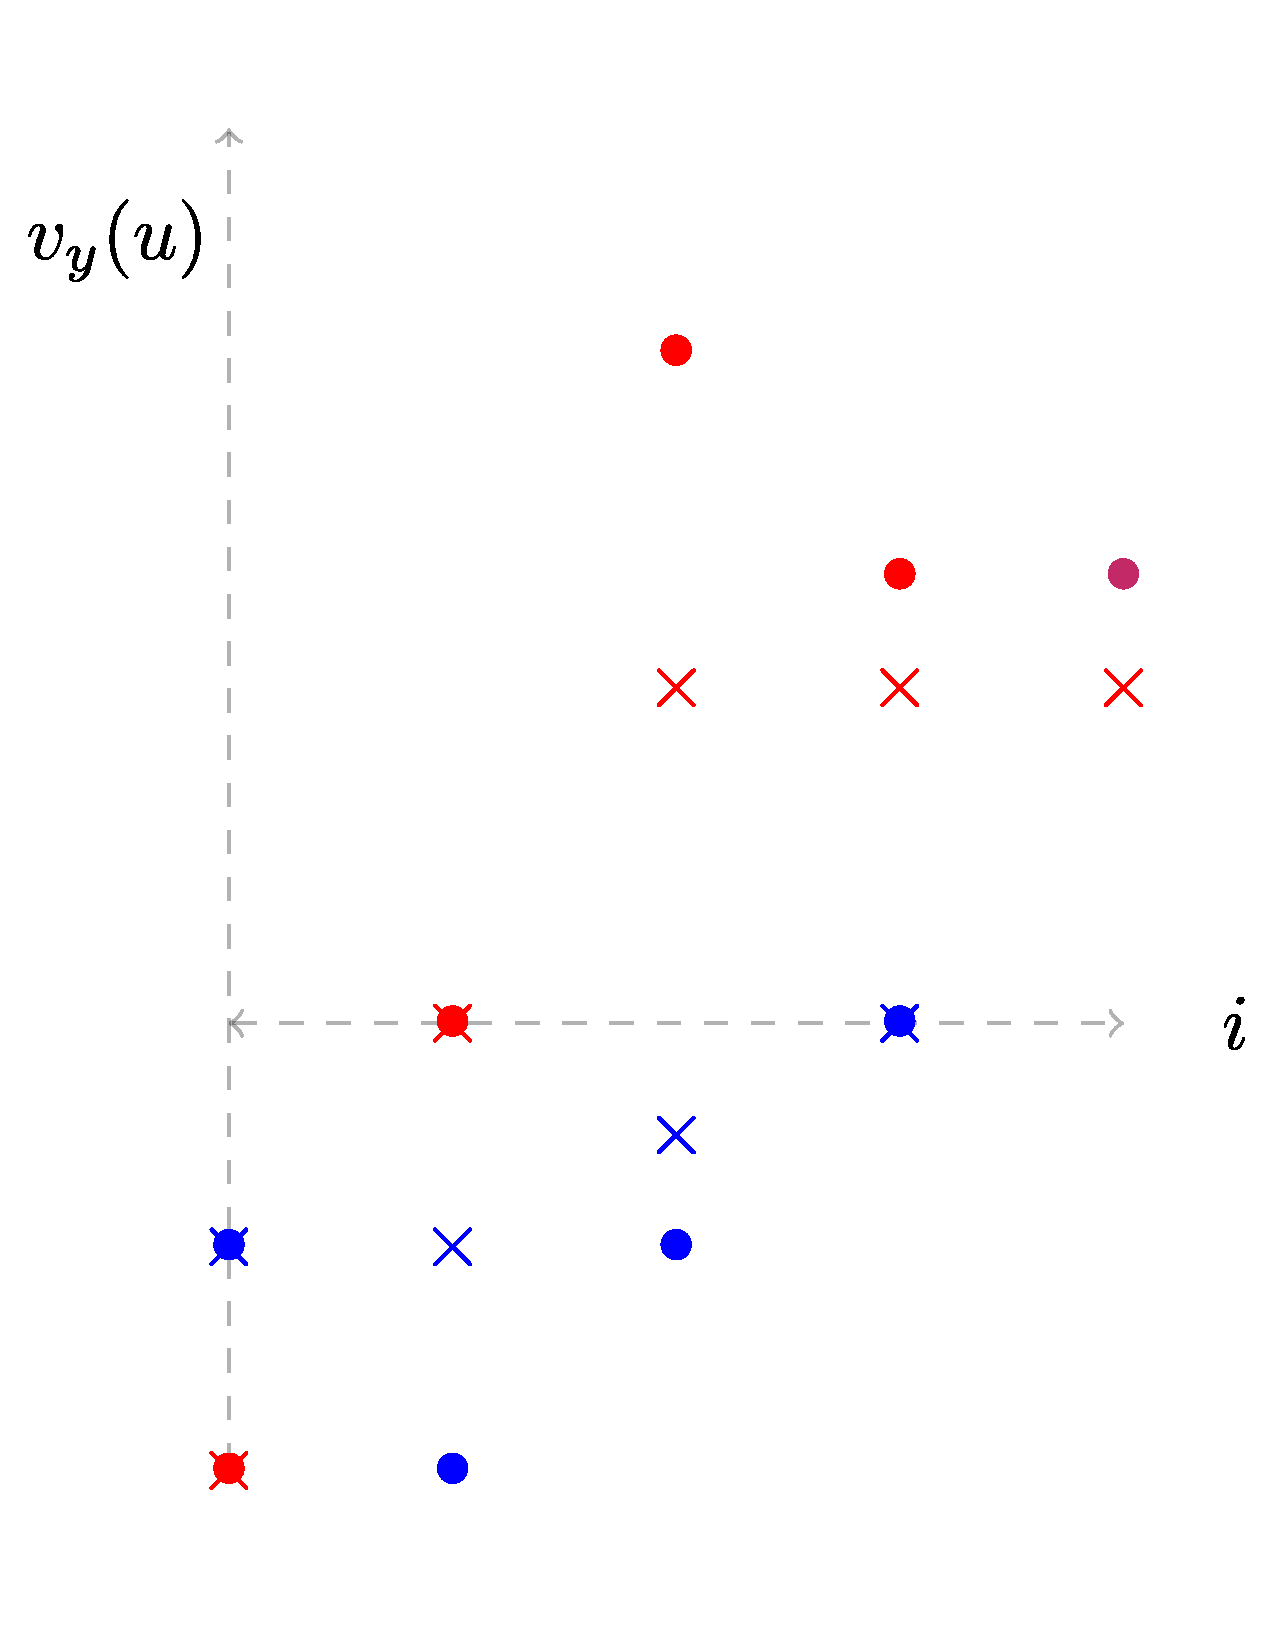
\includegraphics[width=0.7\linewidth]{tikz/real-embed-vs}
	\caption{\textbullet $\;$ represents the original $v_i$, where blue is used for $v(\cdot)_{y_1}$ and red for $v(\cdot)_{y_2}$.  The $\times$ symbol of the same color is the $\Lambda$-corrected directional derivative to force monotonicity.}
	\label{fig:real-embed-vs}	
\end{minipage}
\hfill
\begin{minipage}{0.45\linewidth}
	\centering
	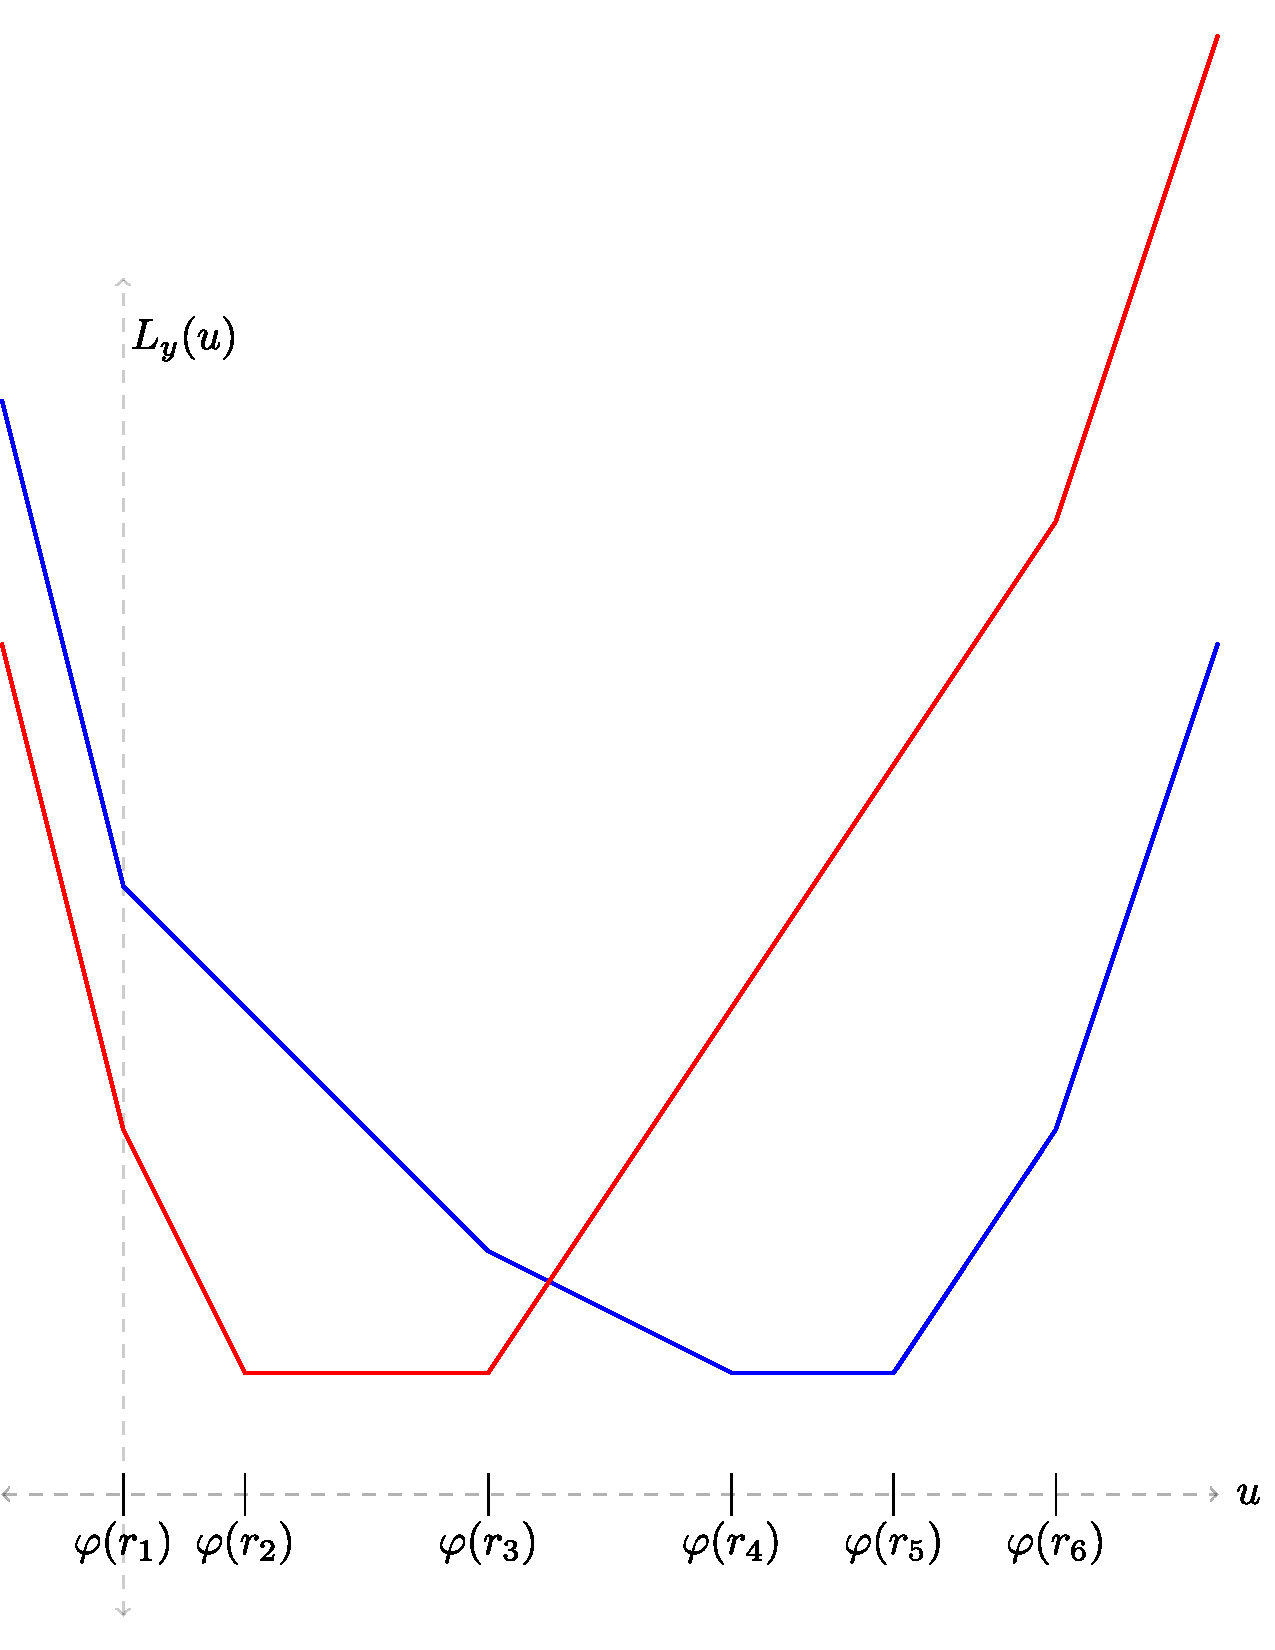
\includegraphics[width=0.7\linewidth]{tikz/real-embed-loss}
	\caption{Our constructed embedding $L$ for the discrete loss $\ell$ given in Table~\ref{tab:example-orderable}.}
	\label{fig:real-embed-loss}
\end{minipage}
\end{figure}

\jessie{If time, write out symbolic calculation}

\section{Polytope notes}
Here, we recall some standard definitions from the theory of Convex Polytopes.
\begin{definition}
	A \emph{polyhedra} in $\reals^d$ is defined by the intersection of a finite number of half-spaces.
	A \emph{polytope} is a bounded polyhedra.
\end{definition}

\begin{definition}[Valid inequality]
	Let $S$ be a set in $\reals^d$.
	A \emph{valid inequality} for $S$ is an inequality that holds for all vectors in $S$.
	That is, the pair $(a,\beta)$ is a valid inequality for $S$ if and only if 
	\begin{align*}
	\inprod{a}{x} &\leq \beta \; \; \forall x \in S~.~
	\end{align*}
\end{definition}

\begin{definition}[Face]\label{def:face}
	For any valid inequality of a polytope, the subset of the polytope of vectors which are tight for the inequality is called a \emph{face} of the polytope.
	That is, the set $F$ is a face of the polytope $T$ if and only if 
	\begin{align*}
	F &= \{x \in T : \inprod{a}{x} = \beta \}
	\end{align*}
	for some valid inequality $(a, \beta)$ of $T$.
\end{definition}

\begin{definition}[Supporting function]
	Let $S$ be a nonempty bounded set in $\reals^d$.
	We call the \emph{supporting function} of $S$ the function $H_S:\reals^d \to \reals$ by
	\begin{align*}
	H_S(a) := \sup_{x \in S}\inprod{a}{x}~.~
	\end{align*} 
\end{definition}

\iffalse
\begin{definition}[Maximizers]
	Let $S \subseteq \reals^d$, and $a \in \reals^d$.
	The \emph{set of maximizers} of $a$ over $S$ is defined as
	\begin{align*}
	\mathcal{S}(S;a) &= \{x \in S : \inprod a x = H_S(a)\}
	\end{align*}
\end{definition}

\begin{definition}[Normal cones]
	Let $T$ be a polytope in $\reals^d$.
	For any face $F$ of $T$, we define its \emph{normal cone} $\N(F;T)$ as the set of vectors for which $F$ is the maximizer set over $T$.
	That is,
	\begin{align*}
	\N(F;T) = \left\{a : F = \mathcal{S}(T; a) \right\}~.~
	\end{align*}
\end{definition}

It is worth noting that normal cones are generally not closed by this definition, but sometimes we may want to think about the closure of the normal cone.
\fi

\begin{definition}[Minkowski sum]
	Let $S_1, S_2, \ldots, S_n$ be sets of vectors.
	We can define their \emph{Minkowski sum} as the set of vectors which can be written as the sum of a vector in each set.
	Namely,
	\begin{align*}
	S_1 \oplus \ldots \oplus S_n &= \{x_1 + \ldots + x_n : x_i \in S_i \; \forall i \}
	\end{align*}
\end{definition}

%\begin{theorem}[\cite[Theorem 3.1.2]{weibel2007minkowski}] \label{thm:unique-face-decomp}
%	Let $T_1, \ldots, T_n$ be polytopes in $\reals^d$ and let $F$ be a face of the Minkowski sum $T := T_1 \oplus \ldots \oplus T_n$.
%	Then there are faces $F_1, \ldots, F_n$ of $T_1, \ldots, T_n$ respectively such that $F = F_1 \oplus \ldots \oplus F_n$.
%	Moreover, this decomposition is unique.
%\end{theorem}

\iffalse 
\begin{corollary}[\cite[Corollary 3.1.3]{weibel2007minkowski}]\label{cor:face-decomp-normal-cones}
	Let $T = T_1 \oplus \ldots \oplus T_n$ be a Minkowski sum of polytopes in $\reals^d$, let $F$ be a nonempty face of $T$ , and let $F_1, \ldots, F_n$ be its decomposition.
	Then $\N(F;T) = \N(F_1;T_1) \cap \ldots \cap \N(F_n; T_n)$.
\end{corollary}

%used in proving completeness of constructed V
\begin{corollary}[\cite[Corollary 3.1.4]{weibel2007minkowski}]
	Let $F_1, \ldots, F_n$ be nonempty faces of the polytopes $T_1, \ldots, T_n$ respectively, then $F_1 \oplus \ldots \oplus F_n$ is a face of $T_1 \oplus \ldots \oplus T_n$ if and only if the intersection of their normal cones is nonempty.
\end{corollary}
\fi

%\begin{theorem}[\cite[Theorem 3.1.6]{weibel2007minkowski}]\label{thm:support-minksum}
%	The supporting function of a Minkowski sum is the sum of the supporting functions of its summands.
%\end{theorem}

\begin{definition}[Weighted Minkowski sum]
	If $T_1, \ldots, T_n$ are polytopes in $\reals^d$, we can call $T(\vec p)$ their \emph{weighted} Minkowski sum for $\vec p \in \reals^n_{\geq 0}$,
	\begin{align*}
	T(\vec p) &:= \oplus_y p_y T_y = p_1 T_1 \oplus \ldots \oplus p_n T_n
	\end{align*}
\end{definition}

%From the thesis:  \emph{``It is easy to see that the normal fan (undefined here, but consequently normal cones) of $p_i T_i$ does not change as long as $p_i$ is positive.  Since the normal fan of a Minkowski sum can be deduced from that of its summands, we can deduce from this that the conbimatorial properties of $\oplus_y p_y T_y$ stay the same as long as all $p_i$ are positive.''}

Suppose we are given a polytope $T_y \in \reals^d$ and set of vectors $V \in \reals^{k \times d}$.
Call $e^y \in \reals^k$ the vector such that $e^y_i = \max_{x \in T_y}\inprod{v_i}{x}$.  
For a finite set $\T = \{T_1, , \ldots, T_n\}$, let us denote the \emph{support matrix} $E = (e^y)_{y=1}^n$.
\begin{definition}
	We say a set of normals $V$ is \emph{complete} with respect to a polytope $T_y$ if $T_y = \{x \in \reals^d: Vx \leq e^y\}$.
\end{definition}
Moreover, we say $V$ is complete with respect to the set of polytopes $\T$ if and only if $V$ is complete with respect to each $T_y \in \T$.

\subsubsection*{Optimality Condition}
In general, we know that $\vec 0$ in the subgradient of $f(r)$ if and only if $r$ is an optimum of convex $f$ in general dimensions.

For nice\footnote{for reports on the relative interior of the domain, and something else} conditions, we have $\vec 0 \in \oplus_i f_i$ if and only if $\vec 0 \in \oplus_i \partial f_i(r)$.
This allows us to consider the following optimality condition:
\begin{definition}\label{def:optimality}[Optimality]
	For all $r \in \R$ and $y \in \Y$, we have $r \in \gamma_r \iff \vec 0 \in \oplus_y p_y T_y(r)$.
\end{definition}
The polytope $T_y(r)$ can be thought of as $\partial L_y(\varphi(r))$.


We will suppose we start with a finite set of $n$ polytopes $\T := \{T_1, \ldots, T_n\}$, and we will call $T := T_1 \oplus \ldots \oplus T_n \in \reals^d$ their Minkowski sum.
We know that every polytope has both a halfspace and vertex representation ($\H$-representation and $\V$-representation, respectively.)
By existence of the $\H$-representation, we know there must be a matrix $V \in \reals^{k \times d}$ and vector $e \in \reals^k$ such that $T = \{x \in \reals^d : Vx \leq e\}$.
In fact, with a complete set of normals $V$, we know that $e$ can be the support vector of each of the normals.
However, finding $V$ is not always easy, so we assume that we are given $V$ for now.

\subsection{Given normals $V$}
Now, for a given polytope $T(p)$, we want to ask when a given $z \in \reals^d$ is in the polytope $T(p)$.
We will later generalize to finding the set of $p \in \simplex$ for which $\vec 0 \in T(p)$ by substituting $z= \vec 0$.
Throughout, assume we have $V$ which is complete for $\T$ and $E$ defined by the support of each normal in $V$ for all $T_y \in \T$.
We denote $e^y = E_{;y}$ as the $y^{th}$ column of $E$, or equivalently, the support vector for $T_y$ given $V$.

Since we define $T_y = \{x : Vx \leq e^y\}$, we can multiply the right side of the inequality by the constant $p_y \geq  0$ to yield $p_y T_y = \{x : Vx \leq p_y e^y\}$.
Taking the Minkowski sum of polytopes described by the same set of normals, we can take 
\begin{align*}
\oplus_y p_y T_y &= \{x : Vx \leq p_1 E_{;1}\} \oplus \ldots \oplus \{x : Vx \leq p_n E_{;n}\} \\
&= \{x : Vx \leq p_1 E_{;1} + \ldots + p_n E_{;n}\}\\
&= \{x : Vx \leq E p\}~.~
\end{align*}
The first to second line follows from Theorem~\ref{thm:support-minksum} and preservation of inequalities under addition.
Now, we have $z \in T(p) \iff \inprod{v_i}{z} \leq (Ep)_i$ for all $v_i \in V$.

Observe that we have $\vec 0 \in T(p)$ if and only if $E p \geq 0$ by substitution, which lines up with our optimality condition in Definition~\ref{def:optimality}.  

We assume $p \in \simplex$, so we now describe the cell $D^\T := \{p \in \simplex : Ep \geq \vec 0\}$ as the set of distributions such that $\vec 0 \in T(p)$.
In cases where $\T$ is obvious from context, we omit the subscript and just write $D$.

Given the complete set of normals $V$ and constructing the support matrix for $V$ and $\T$, $E$, we observe that $E$ is unique up to rescaling.
However, as discussed earlier, there are always multiple complete sets of normals for $\T$, and so in that sense, $E$ is not unique.

\subsection{Equivalences}
In the big picture, we want to know two things.
First, if we are given a cell $C$, how we can construct a finite set of polytopes $\T = \{T_1, \ldots, T_n\}$ such that $\vec 0 \in T(p) \iff p \in C$.
Second, we want to know the opposite case: starting from $\T$, can we derive the cell $C \subseteq \simplex$ where $\vec 0 \in T(p)$ for all $p \in C$?
We start with the latter, leaving the former for future work.

We know that if we are given $\T$ and a complete set of normals $V$, we can describe $D = \{p \in \simplex : Ep \geq \vec 0\}$ as in Section~\ref{sec:start-polytope}.
However, we do not necessarily have $D' := \{p \in A : Ep \geq \vec 0\} \subseteq \simplex$, and this poses some issues given the construction of the cell $C$ only assuming that we are in the affine span of the simplex, but not necessarily in the simplex.

\begin{lemma}\label{lem:describe-D}
	Suppose we are given polytopes $\T = \{T_1, \ldots, T_n\}$ and a set of normals $V$ that is complete for $\T$.
	Take $E = (e_{i}^y)$ where $e_{i}^y = \max_{x \in T_y} \inprod{v_i}{x}$, and $D^\T = \{p \in \simplex : Ep \geq \vec 0\}$.
	
	Then $\{p \in \simplex : \vec 0 \in \oplus_y p_y T_y\} = \{p \in \simplex: Ep \geq \vec 0\}$.\btw{on the whiteboard: ``stuff about $E$ and $D$.''}
\end{lemma}
\begin{proof}
	First, let us fix a distribution $p \in \simplex$.
	By Theorem~\ref{thm:support-minksum}, we have the support of the (weighted) Minkowski sum is the (weighted) sum of the support of each polytope, which we can re-write the weighted support as the product $Ep$.
	
	Each halfspace is bounded by the support function of the weighted polytope by construction of $E$, so the support of the weighted polytope defined by an inequality on $v_i$ can be described as $\inprod{v_i}{z} \leq \inprod{E_i}{p}$.
	Taking this for all $v_i$, we then have $\oplus_y p_y T_y = \{x \in \reals^d : Vx \leq Ep\}$.
	
	Therefore, for fixed $p$, we have $\vec 0 \in \oplus_y p_y T_y \iff Ep \geq \vec 0$.
	As $p \in \simplex$ was arbitrary, we observe the stated set equality.
\end{proof}

\begin{proposition}\label{prop:relate-E-B}
	Suppose we are given polytopes $\T = \{T_1, \ldots, T_n\}$ and a set of normals $V$ that is complete for $\T$.
	Take $E = (e_{iy})$ where $e_{iy} = \max_{x \in T_y} \inprod{v_i}{x}$, and take $D = \{p \in \simplex : Ep \geq \vec 0\}$ and take the minimal rank $B \in \reals^{k \times n}$ such that we have the given cell $C = \{p \in \simplex : Bp \geq \vec 0\}$.
	
	Then $\{p \in \simplex : \vec 0 \in \oplus_y p_y T_y\} = C$	if and only if $C = D$.
\end{proposition}
\begin{proof}
	By Lemma~\ref{lem:describe-D}, we have $D = \{p \in \simplex : \vec 0 \in \oplus_y p_y T_y\}$, and the result follows.
\end{proof}

\begin{definition}
	We say a vector $v$ is \emph{redundant} with respect to matrix $Y$ if we have $\{z: Yz \geq \vec b\} = \{z : [Y;v]z \geq \vec b^*\}$, where $b^* = [b;c]$ for some constant $c \in \reals$.
\end{definition}

\begin{proposition}\label{prop:relate-rows}
	Suppose we have polytopes $\T = \{T_1, \ldots, T_n\}$ and a set of normals $V$ that is complete for $\T$.
	Take $E = (e_{i}^y)$ where $e_{i}^y = \max_{x \in T_y} \inprod{v_i}{x}$, and take $D = \{p \in \simplex : Ep \geq \vec 0\}$ and take the minimal matrix $B$ such that a given cell $C = \{p \in \simplex : Bp \geq \vec 0\}$.
	
	Then $\{p \in \simplex : \vec 0 \in \oplus_y p_y T_y\} = C$	if and only the rows of $B$ appear in $E$ (possibly scaled) and every other row of $E$ is redundant with respect to $B$.
	\btw{``replace prop 1 statement with `non-simplex rows of $B$ appear in $E$ (possible scaled) and every other row of $E$ is redundant with respect to $B$.'''}
\end{proposition}
\begin{proof}
	\begin{itemize}
		\item [$\implies$] First, assume $C = \{p \in \simplex: \vec 0 \in \oplus_y p_y T_y\}$.
		By Proposition~\ref{prop:relate-E-B}, we know that $C = D^\T := \{p \in \simplex : Ep \geq \vec 0\}$.
		Then we have $\{p \in \simplex : Bp \geq \vec 0\} = \{p \in \simplex : Ep \geq \vec 0\}$.
		As $B$ is minimal, we must have that every row of $B$ appears (possibly scaled) in $E$.
		Otherwise, we would contradict equality of the polytopes $C$ and $D$.
		Moreover, all rows in $E$ not in $B$ are redundant with respect to $B$ by equality of the polytopes.
		
		
		\item [$\impliedby$] Suppose that all rows of $B$ appear in $E$, and every other row of $E$ is redundant with respect to $B$.
		Then we have $D = \{p\in \simplex : Ep \geq \vec 0\} = \{p \in \simplex : Bp \geq \vec 0\} = C$.
		
		Then $D = C$, and by Proposition~\ref{prop:relate-E-B}, we have $C = \{p \in \simplex : \vec 0 \in \oplus_y p_y T_y\}$.
	\end{itemize}
\end{proof}


\section{$d$-dimensional omitted proofs}\label{app:omitted-d-dim}
\begin{proof}[Proof of Lemma~\ref{lemma:minkowski-support}]
	\jessie{Appendix}
	For each $p$, $\oplus_p \T$ is a polytope.
	\bo{TODO: it turns out that $p$ doesn't matter, only its support; and there are only finitely many possible supports (or even better, the normals that are complete for the uniform minkowski sum turn out to be complete for all other $p$-combinations).}
	For each of the finitely many supports ($2^n - 1$), we know $\oplus_p \T$ is a polytope, and every polytope can be uniquely defined by an enumeration of vectors normal to its facets.
	As a two polytopes with the same support can be defined by the same facet enumeration, we can simply concatenate these finite set of normals for the finite polytope supports.
	Vectors that are not normal to a facet simply become redundant constraints.
	This yields finitely many normals defining the weighted Minkowski sum $\oplus_p \T$ for all $p \in \simplex$.
\end{proof}

\begin{proof}[Proof of Lemma~\ref{lemma:D-polytope}]
	\jessie{Appendix}
	Recall by definition, the notation $\oplus_p \T = \{\sum_y p_y x_y : x_y \in T_y (\forall y)\}$.
	Each $T_y$ is a polytope, so $p_y T_y$ is a polytope.
	The Minkowski sum of polytopes is a polytope, so $\oplus_p \T$ is a polytope by~\cite[Section 1.2]{weibel2007minkowski}.
	\bo{TODO}\jessie{Taking a try}
	Since $\oplus_p \T$ is a polytope for all $p \in \simplex$, we know there is a halfspace representation of normals $V$ so that for all $y \in \Y$, we have $x \in p_yT_y \iff \inprod{V}{x} \leq p_y e^y$ for some matrix $V$ and the support vector $e^y$, where $e^y_i = H_{T_y}(V_i)$.
	Adding redundant constraints for the $e^y$ as necessary, we know that the support of the Minkowski sum for a given normal is the sum of the normals~\cite[Theorem 3.1.6]{weibel2007minkowski}.
	Concatenating the vectors $e^y$ into $E$, we have $x \in \oplus_p \T \iff \inprod{V^*}{x} \leq E^*p$, where $V^*$ has redundant rows added as necessary. \jessie{Hand wavy... not a fan.}
	Substituting $x = \vec 0$, we see $\vec 0 \in \oplus_p \T \iff Ep \geq \vec 0$, which defines a polytope by construction of $E$.
\end{proof}

\begin{proof}[Proof of Lemma~\ref{lemma:E-to-B}]
	\bo{? Cite} \jessie{Is left as an exercise in the following text:} \cite[Exercise 2.15]{ziegler2012lectures}
\end{proof}


\section{Simplifying the QFP for $\abstain{1/2}$, $d=2$}
In order to prove Proposition~\ref{prop:qfp-fails-abstain}, we take some simplifying steps to the quadratic feasibility program for this specific problem.
The strategy is to consider the level set $\gamma_{\bot}$, the set of distributions with modal mass at most $1/2$.
We show that the quadratic feasibility program with this input cannot be satisfied with dimension $2$ for $n=5$.

\begin{lemma} \label{lemma:abstain-v-h}
	For the abstain loss $\ell_{1/2}$, the level set of abstain satisfies $\gamma_{\bot} = \conv\{(\delta_y + \delta_{y'})/2 : y,y' \in \Y, y < y'\} = \{p : Bp \geq \vec{0}\}$ where $\delta_y$ puts probability one on $y$ and $B = \ones \ones^{\intercal} - 2I \in \reals^{5 \times 5}$, i.e. has entries $-1$ on the diagonal and $1$ everywhere else.
\end{lemma}
\begin{proof}
	Recall that $\gamma_{\bot}$ is the set of distributions $p$ with $\max_y p_y = 1/2$.
	First, note that each distribution of the form $(1/2, 1/2, 0, 0, 0)$ and so on is in $\gamma_{\bot}$.
	Meanwhile, every such $p$ can be written as a convex combination of these corners.
	Second, note that if $p \in \gamma_{\bot}$, then $p_y \leq 1/2$ for all $y \in \Y$.
	These constraints can be rewritten as $\inprod{p}{b} \geq 0$ where $b_y = -1$ and $b_{y'} = 1$ for all $y' \neq y$, literally requiring $p_y \leq \sum_{y' \neq y} p(y')$.
\end{proof}

\begin{observation} \label{obs:qfp-invariant-lin}
	For any invertible $A \in \reals^{d \times d}$, if $V,\{X^j : j \in [\ell]\}$ is a feasible solution to the quadratic feasibility program, then so is $(VA),\{A^{-1}X^j : j \in [\ell]\}$.
\end{observation}
\begin{proof}
	The halfspace constraints are $(VA)(A^{-1}X^j) \leq B \iff VX^{j} \leq B$.
	The $j^{th}$ vertex constraint is a vector equality $\sum_{y \in \Y} p^j(y) (A^{-1}X^j)_y = \vec{0}$.
	If we let $a_m$ be the $m^{th}$ row of $A^{-1}$, then the $m^{th}$ row of the vector equality is
	\begin{align*}
	0 &= \sum_{y \in \Y} p^j(y) \inprod{a_m}{x^j_y}  \\
	&= \inprod{a_m}{\sum_{y \in \Y} p^j(y) x^j_y}  \\
	&= 0
	\end{align*}
	so the program is feasible.
\end{proof}

\begin{corollary} \label{cor:qfp-wlog-v1}
	If there is a feasible solution to the quadratic feasibility program, then there is a feasible solution where $v_1$ is the first standard basis vector and $\|v_i\| \leq \|v_1\| = 1$ for all $i$.
\end{corollary}
\begin{proof}
	In particular, we can take a series of matrices $A$ in Observation \ref{obs:qfp-invariant-lin} that permute the rows of $V$, scale\footnote{Note one can show $V = 0$ is not feasible unless $B$ is a trivial property, i.e. essentially has no rows at all.} all rows by $\frac{1}{\|v_1\|}$, and linearly map $v_1$ to $(1,0,\dots,0)$.
\end{proof}

\paragraph{Notation for the quadratic program.}
Recall that in the quadratic program, each vertex $p$ in the convex-hull representation corresponds to a matrix variable $X$.
Here, the vertices are indexed by a pair of distributions, so for each $i < j$, we refer to that vertex of $\gamma_{\bot}$ by $p^{ij} = (\delta_i + \delta_j)/2$, with corresponding variable $X^{ij}$.
The $y$th column of this matrix is denoted $x^{ij}_y \in \reals^d$.
%Specifically, for the $\ellabs{\alpha}$, we denote $X^m$ by $x^{ij}$, where $p^m$ is the distribution of support $2$ putting weight $1-\alpha$ on outcome $i$, and weight $\alpha$ on outcome $j$.
%As the convex hull of a finite number of these distributions can be used to describe the abstain cell, we can simplify our QFP by studying these elements of the $X$ matrix, and getting rid of each other $x^{ij}_q$, for $q \neq i,j$, since these do not appear in the constraints.
%Observe that each $x^{ij}$ is a matrix, and we denote $x^{ij}_i$ as the $i^{th}$ column\jessie{?} of the matrix $x^{ij}$.
%When we look at a specific inner product, then we have $\inprod{v_i}{x^{ij}_y} \leq B_{iy}$.
%\jessie{With how I wrote this, might be helpful to index the QFP with $m$.  Feel free to change though.}

\begin{lemma} \label{lemma:xiji-minus-xijj}
	In any feasible solution to the QFP for $\gamma_{\bot}$ and $\ell_{1/2}$, we have $x^{ij}_i = -x^{ij}_j$ for all $i<j$ in $\Y$.
\end{lemma}
\begin{proof}
	Directly from the vertex constraints: $p^{ij} = \frac{1}{2}\delta_i + \frac{1}{2}\delta_j$, so the $ij$ constraint reduces to $\frac{1}{2}x^{ij}_i + \frac{1}{2}x^{ij}_j = \vec 0$.
\end{proof}

\begin{lemma} \label{lemma:vi-neq-cvj}
	There is no feasible solution to the QFP for $\gamma_{\bot}$ and $\ell_{1/2}$ where $v_i = c v_j$ for $c > 0$ and any $i \neq j$.
\end{lemma}
\begin{proof}
	There is an open halfspace through the origin strictly containing both the feasible regions $F_i = \{x : \inprod{v_i}{x} \leq -1, \inprod{v_j}{x} \leq 1 \; \forall j \neq i\}$ and $F_j$, so there is no set of witnesses such that $x^{ij}_i \in F_i$ and $x^{ij}_j \in F_j$, as this would contradict Lemma \ref{lemma:xiji-minus-xijj}.
\end{proof}

\begin{lemma} \label{lemma:unique-spot-xiji}
	For $d=2$ and the level set $\gamma_\bot$ for $\ell_{1/2}$, any pair of linearly independent $v_i,v_j$ rule out all except for a unique feasible value for $x^{ij}_i$ and also for $x^{ij}_j$.
\end{lemma}
\begin{proof}
	From the halfspace constraints, we must have $\inprod{v_i}{x^{ij}_i} \leq -1$ and $\inprod{v_i}{x^{ij}_j} \leq 1$, which combines with Lemma \ref{lemma:xiji-minus-xijj} to give $\inprod{v_i}{x^{ij}_i} = 1$.
	This immediately also gives $\inprod{v_j}{x^{ij}_i} = -1$.
	This system of two inequalities in two dimensions has exactly one solution if $v_i,v_j$ are linearly independent.
\end{proof}

\begin{figure}
	\begin{minipage}{0.45\linewidth}
		\centering
		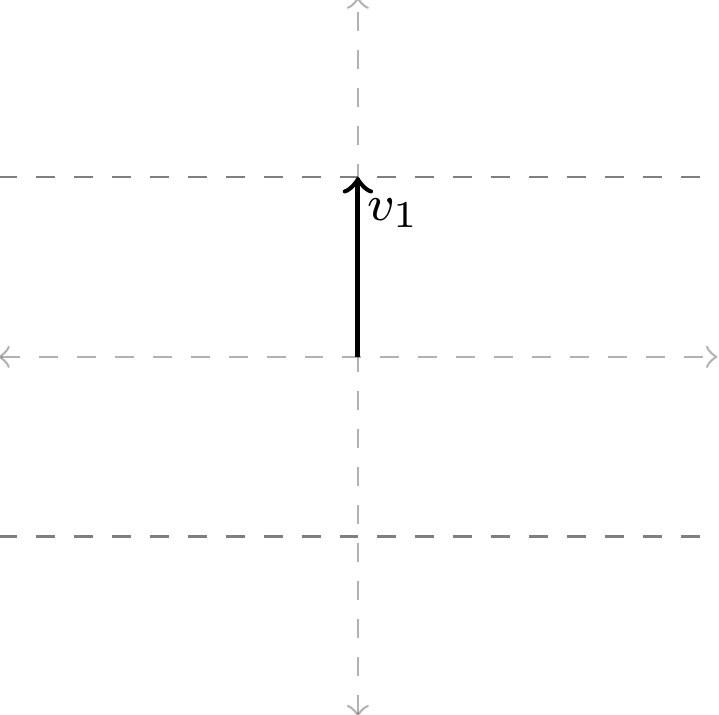
\includegraphics[width=0.9\linewidth]{tikz/v1}
		\caption{Example of $v_1$.}
		\label{fig:v1}
	\end{minipage}
	\hfill
	\begin{minipage}{0.45\linewidth}
		\centering
		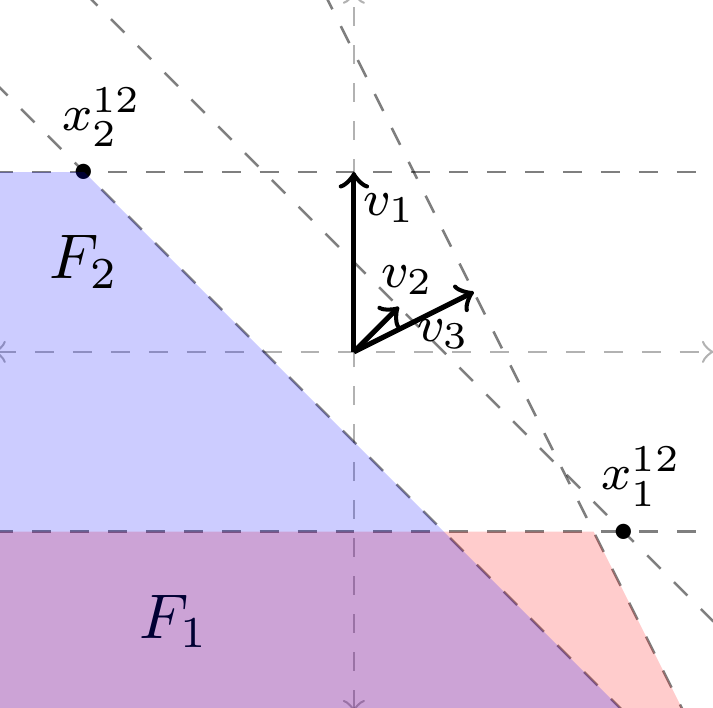
\includegraphics[width=0.9\linewidth]{tikz/qp-must-intersect-line-same-spot}
		\caption{If $x^{12}_1 \neq x^{13}_1$, we have a contradiction.}
		\label{fig:qp-must-intersect-line-same-spot}
	\end{minipage}
\end{figure}
\begin{figure}
		\begin{minipage}{0.4\linewidth}
		\centering
		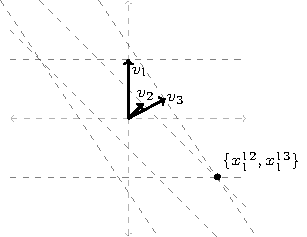
\includegraphics[width=0.9\linewidth]{tikz/qp-intuition-contradiction.pdf}
		\caption{Reducing to the case where $x^{12}_1 = x^{13}_1$.}
		\label{fig:qp-line-intersect-contradiction}
	\end{minipage}
\hfill
	\begin{minipage}{0.59\linewidth}
	\centering
	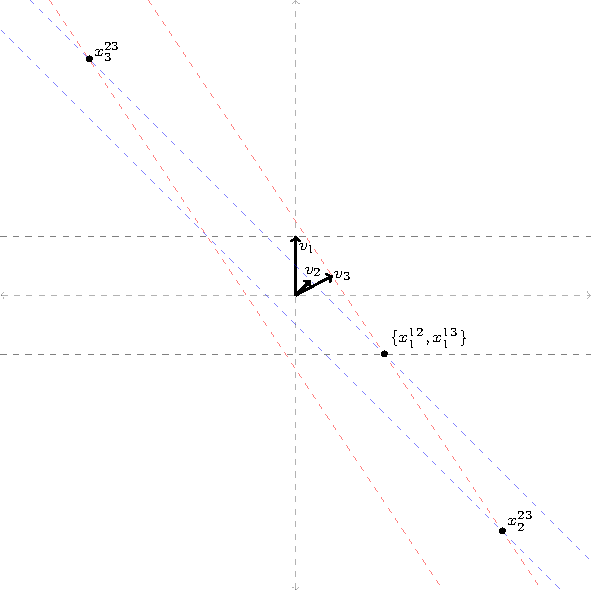
\includegraphics[width=0.9\linewidth]{tikz/qp-intuition-contradiction-with-intersection.pdf}
	\caption{The intersection of $\inprod{v_2}{x} = -1$ and $\inprod{v_3}{x} = 1$ occurs outside the region $\inprod{v_1}{x} \in [-1,1]$.}
	\label{fig:qp-line-intersect-contradiction-with-intersection}
	\end{minipage}
\end{figure}

\begin{lemma} \label{lemma:180-degree-no-three}
	There is no feasible solution to the QFP for $\gamma_{\bot}$ and $\ell_{1/2}$ where three vectors $v_i,v_j,v_m$ lie strictly within a halfspace through the origin (i.e. all within $180^{\circ}$ of each other).
\end{lemma}
\begin{proof}
	Let three of the vectors be given, lying strictly inside a halfspace, and label them clockwise as $v_1,v_2,v_3$.
	WLOG suppose $v_1$ points vertically ``up'', as in Figure \ref{fig:v1}.
	By Lemma \ref{lemma:unique-spot-xiji}, the possible locations of the following points are all uniquely determined: $x^{ij}_i, x^{ij}_j$ for $(i,j) \in \{(1,2),(1,3),(2,3)\}$.
	Both points $x^{12}_1$ and $x^{13}_1$ lie on the line $\inprod{v_1}{x} = -1$, i.e. a horizontal line below the origin.
	We have constraints $\inprod{v_2}{x^{12}_1} = 1$ and $\inprod{v_2}{x^{13}_1} \leq 1$.
	This implies $x^{13}_1$ is left of $x^{12}_1$ on the horizontal line $\inprod{v_1}{x} = 1$. 
	But the symmetric constraints $\inprod{v_3}{x^{13}_1} = 1$ and $\inprod{v_3}{x^{12}_1} \leq 1$ imply symmetrically that $x^{12}_1$ is left of $x^{13}_1$ on the line.
	This implies we must have $x^{12}_1 = x^{13}_1$.
	
	If we consider the four lines $\inprod{v_2}{x}=1, \inprod{v_2}{x}=-1, \inprod{v_3}{x}=1, \inprod{v_3}{x}=-1$, we therefore have three points of intersection with the line $\inprod{v_1}{x}=1$ and three with the line $\inprod{v_1}{x}=-1$. 
	WLOG, these points from top left to top right are: $x^{12}_2$ (which equals $x^{13}_3$), the intersection with $\inprod{v_2}{x}=1$, and the intersection with $\inprod{v_3}{x}=1$; and therefore from bottom left to bottom right are: the intersection with $\inprod{v_3}{x}=-1$, the intersection with $\inprod{v_2}{x}=-1$, and the intersection with $x^{12}_1$ (which equals $x^{13}_1$).
	\bo{Needs more justification why these points are always in this order (up to renaming of $v_2$ and $v_3$).}\jessie{Should we be able to take these to be in clockwise order WLOG in the grand scheme of trying to pack 5 normals into 180 degrees?  The order of the intersections follows from the clockwise order of the normals.  (ex: if the order was $v_2, v_1, v_3$, we would still get a contradiction, but in the first case like Figure~\ref{fig:intersection-graph-ex} I think)}
	
	This implies that the lines $\inprod{v_2}{x}=-1$ and $\inprod{v_3}{x}=1$, in particular, do not intersect anywhere within the bounds of $\inprod{v_1}{x} \in [-1,1]$.
	Therefore, either their intersection point $x^{23}_2$ or its negative $x^{23}_3$ violates the feasibility constraint $\inprod{v_1}{x} \leq 1$.
	This proves there is no feasible solution with three normals lying strictly in the same halfspace through the origin.
\end{proof}

\begin{proposition}
	The abstain loss $\ell_{1/2}$ with $n=5$ is not $2$-embeddable.
\end{proposition}
\begin{proof}
	Let any $5$ vectors be given, numbered clockwise.
	$v_1,v_2,v_3$ cannot lie in a cone of strictly less than $180^{\circ}$, as this would contradict Lemma~\ref{lemma:180-degree-no-three}.
	So the clockwise angle between $v_1$ and $v_3$ is at least $180^{\circ}$.
	Since there are no duplicate angles (Lemma \ref{lemma:vi-neq-cvj}), this implies that the clockwise angle between $v_4$ and $v_1$, which includes $v_5$, is strictly less than $180^{\circ}$.
	This contradicts Lemma~\ref{lemma:180-degree-no-three}.
\end{proof}

%\begin{proposition}
%	The abstain loss $\ell_{1/2}$ with $n=5$ is not $2$-embeddable.
%\end{proposition}
%\begin{proof}[Geometric proof]
%  We apply Corollary \ref{cor:d-embeddable-char}: We consider the level set $\gamma_{\bot}$ (the distributions whose modal mass is at most $1/2$).
%  We show that the quadratic program (Definition \ref{def:qfp}) is not feasible for this polytope with dimension $d=2$, which implies by Corollary \ref{cor:d-embeddable-char} that $\ell$ is not $2$-embeddable.
%
%  We obtain the vertex and halfspace representations of $\gamma_{\bot}$ from Lemma \ref{lemma:abstain-v-h}.
%  We proceed by narrowing the space of feasible normals $v_1, \ldots, v_5$, until we reach a contradiction.
%  %We make an argument on the permissible angles between normals $v_1, \ldots, v_5$ in $\reals^2$ and show there is no feasible solution to the QFP in Definition~\ref{def:qfp}.
%  In particular, we argue that in any cone strictly $ < 180^\circ$, we can have no more than two vectors $v_i$ and $v_j$; otherwise we yield a contradiction.
%
%  We index the vertices and witnesses as follows: For $y < y'$, we write $p^{yy'} = (\delta_y + \delta_{y'})/2$ and $X^{yy'}$ for the corresponding matrix variable, with columns (witness points) $x^{yy'}_{y''}$.
%  In particular, the vertex constraints can all be rearranged to yield the following: $\{x^{yy'}_y = -x^{yy'}_{y'} ~ (\forall y < y')\}$.
%  Our proof will ignore all other points, i.e. $x^{yy'}_{y''}$ for $y'' \neq y,y'$, which appear only with coefficient zero in the vertex constraints.
%
%  Without loss of generality, we let $v_1 = (0,1)$, and have $v_2$ with $\|v_2\|^2 \leq \|v_1\|^2$ and the angle $\theta_{12} < 180^\circ$ the angle between $v_1$ and $v_2$. \bo{Need to justify why choice of $v_1$ is WLOG.}
%
%  We then have the feasible regions $F_y = \{x \in \reals^2 : \inprod{v_i} {x} \leq B_{iy} \; \forall i\}$, which means to this point, we have $F_1 = \{x \in \reals^2 : \inprod{v_1}{x} \leq -1 \text{ and } \inprod{v_2}{x} \leq 1 \}$, and $F_2 = \{x \in \reals^2 : \inprod{v_1}{x} \leq 1 \text{ and } \inprod{v_2}{x} \leq -1 \}$.
%  By requirement of the existence of a set of witnesses for the distribution $(1/2, 1/2, 0,0,0)$, we must have some $x^{12}_1 \in F_1$ and $x^{12}_2 \in F_2$ so that $x^{12}_1 = -x^{12}_2$ in order for $\vec 0$ to be in the Minkowski sum.
%  In particular, we know that, since $\theta_{12} < 180^\circ$, $x^{12}_1$ and $x^{12}_2$ are unique given $v_1$ and $v_2$.
%
%  We then want to show that we cannot add a $v_3$ such that $\max(\theta_{12}, \theta_{13}, \theta_{23}) < 180^\circ$ without yielding a contradiction, which then gives our result, as any arrangement of $5$ normals in $\reals^2$ must have some cone that is less than $180^\circ$ containing three normals.
%
%  In general, observe that $x^{12}_1$ and $x^{13}_1$ must both be on the line $\inprod{v_1}{x} = -1$. \jessie{More detail}
%  Therefore, our three cases proceed as follows: $(i.) \|x^{13}_1\| > \|x^{12}_1\|$, $(ii.) \|x^{13}_1\| = \|x^{12}_1\|$, and $(iii.) \|x^{12}_1\| > \|x^{13}_1\|$.
%  As the labels on normals $v_2$ and $v_3$ (and therefore, the respective witnesses) are arbitrary, it suffices to just show cases $(i.)$ and $(ii.)$.
%
%  \begin{enumerate}
%  \item [$(i.)$] First, suppose $\|x^{13}_1\| < \|x^{12}_1\|$.
%  This in turn implies that $\|v_3\| > \|v_2\|$ since both witnesses are on the line $\inprod{v_1}{x^{1i}_1} = -1$.
%  Consider that in order for $x^{12}_1 \in F_1$, we must have both $\inprod{v_2}{x^{12}_1} = 1$ and $\inprod{v_3}{x^{12}_1} \leq 1$.
%    \begin{align*}
%    \inprod{v_2}{x^{12}_1} = 1 &\iff \|v_2\| \cos(\theta(v_2, x^{12}_1)) = \frac 1 {\|x^{12}_2\|}\\
%    \inprod{v_3}{x^{12}_1} \leq 1 &\iff \|v_3\| \cos(\theta(v_3, x^{12}_1)) \leq \frac 1 {\|x^{12}_2\|}\\
%\implies \|v_3\| \cos(\theta(v_3, x^{12}_1)) &\leq \|v_2\| \cos(\theta(v_2, x^{12}_1))\\
%\implies 1 < \frac{\|v_3\|}{\|v_2\|} &\leq \frac{\cos(\theta(v_2, x^{12}_1))}{\cos(\theta(v_3, x^{12}_1))}\\
%\implies \theta(v_3, x^{12}_1) &> \theta(v_2, x^{12}_1)\\
%\implies \theta_{13} < \theta_{12}
%    \end{align*}
%    This yields a contradiction, as we must have $\theta_{12} < \theta_{13}$ in order to have $\inprod{v_3}{x^{13}_1} = \inprod{v_2}{x^{12}_1} = 1$.
%    Therefore, we conclude that we cannot have $\|x^{12}_1\| > \|x^{13}\|$.
%  	\item [$(ii.)$] Suppose that we have $\|x^{12}_1\| = \|x^{13}_1\|$.
%  	As both witnesses are on the same halfspace $\{x : \inprod{v_1}{x} = -1\}$, we must have $x^{12}_1 = x^{13}_1$.
%
%  \end{enumerate}
%
%%  We do this by arguing that in all three cases of the argmax, we either restrict $F_1$ so that $x_1 \not \in F_1$, restrict $F_2$ so that $x_2 \not \in F_2$, or have $x_3 \not \in F_3$.
%%  We merge the latter two cases without loss of generality as we can relabel these normals pretty easily because of the structure of $B$.
%%
%
%%
%%  \begin{enumerate}
%%  	\item [$\theta_{23} = \argmax$]
%%  	Since $\theta_{23} < 180^\circ$ and $v_1$ is in the middle of $v_2$ and $v_3$, we have that $x^{12}_1 \neq x^{13}_1$.
%%  	Without loss of generality, suppose $\|v_2\|^2 \leq \|v_3\|^2$.
%%  	Then we claim that $x^{13}_1 \not \in F_1$, since we have $x^{13}_1 = \{x : \inprod{v_1}{x} = -1 \text{ and } \inprod{v_3}{x} = 1\}$.
%%  \end{enumerate}
%
%\end{proof}
\begin{proof}[Matrix rank proof of Proposition~\ref{prop:qfp-fails-abstain}]
	We can formulate the QFP given in Section~\ref{sec:d-dim} for $\abstain{1/2}$ as a matrix rank problem.
	First, as observed in Lemma \ref{lemma:xiji-minus-xijj}, the vertex constraints are exactly equivalent to requiring that, in our notation, $x^{ij}_i = - x^{ij}_j$ for all $i<j$.
	Therefore, we can substitute in for all variables of the form $x^{ij}_j$ and eliminate them from the problem.
	Second, we can observe that the program is only easier to satisfy if one drops the halfspace constraints on all variables of the form $x^{ij}_m$, $i < j$, $m \not\in \{i,j\}$.
	This allows us to drop all such variables, and we are now left with only the variables $v_1,\ldots,v_k$ and $\{x^{ij}_i : i<j\}$, with the understanding that $x^{ij}_j = -x^{ij}_i$.
	We can therefore simplify the following constraints of the QFP:
	\begin{align*}
	\inprod{v_i}{x^{ij}_i} &\leq B_{ii} = -1   \\
	\inprod{v_i}{x^{ij}_j} &\leq B_{ij} = 1  \\
	\implies \inprod{v_i}{x^{ij}_i} &= -1  \\
	\inprod{v_i}{x^{ji}_i} &\leq B_{ii} = -1  \\
	\inprod{v_i}{x^{ji}_j} &\leq B_{ij} = 1  \\
	\implies \inprod{v_i}{x^{ji}_j} &= 1  \\
	\inprod{v_i}{x^{jm}_j} &\leq B_{ij} = 1  \\
	\inprod{v_i}{x^{jm}_m} &\leq B_{im} = 1  \\
	\implies \inprod{v_i}{x^{jm}_j} &\in [-1,1] .
	\end{align*}
	
	This gives us the following simplified feasibility problem.
	\begin{align*}
	\inprod{v_i}{x^{ij}_i} &= -1     & (\forall i<j)  \\
	\inprod{v_i}{x^{ji}_j} &= 1      & (\forall i<j)  \\
	\inprod{v_i}{x^{jm}_j} &\in [-1,1]   & (\forall j<m, i\not\in\{j,m\}) .
	\end{align*}
	If we consider the matrix $V$ and construct $Y$ whose columns are $\{x^{ij}_i : i<j\}$, this problem asks us to find such a $V$ and $Y$ whose product $M = VY$ is a matrix with certain fixed entries and others bounded.
	
	In particular, with $n=4$, we obtain the following matrix rank problem: does there exist
	\[
	M_4 = 
	\begin{bmatrix}
	-1 & -1 & -1 & \cdot & \cdot & \cdot \\
	1 & \cdot & \cdot & -1 & -1 & \cdot \\
	\cdot & 1 & \cdot & 1 & \cdot & -1 \\
	\cdot & \cdot & 1 & \cdot & 1 & 1 \\
	\end{bmatrix}
	\]
	where each unknown entry $\cdot$ is in $[-1,1]$, of rank $d=2$?
	
	Since $M_4$ is a submatrix of the matrix obtained when $n=5$, any rank-$2$ solution for the large matrix given below must also solve the above problem.
	
	\[
	M_5 =
	\begin{bmatrix}
	{\color{red} -1} & {\color{red} -1} & {\color{red} -1} & {\color{red} \cdot} & {\color{red} \cdot} & {\color{red} \cdot} & -1 & \cdot & \cdot & \cdot \\
	{\color{red} 1} & {\color{red} \cdot} & {\color{red} \cdot} & {\color{red} -1} & {\color{red} -1} & {\color{red} \cdot} & \cdot & -1 & \cdot & \cdot \\
	{\color{red} \cdot} & {\color{red} 1} & {\color{red} \cdot} & {\color{red} 1} & {\color{red} \cdot} & {\color{red} -1} & \cdot & \cdot & -1 & \cdot \\
	{\color{red} \cdot} & {\color{red} \cdot} & {\color{red} 1} & {\color{red} \cdot} & {\color{red} 1} & {\color{red} 1} & \cdot & \cdot & \cdot & -1 \\
	\cdot & \cdot & \cdot & \cdot & \cdot & \cdot & 1 & 1 & 1 & 1\\
	\end{bmatrix}
	\]
	
	\bo{I'm not sure the below is a proof, because you could have linear combinations with any coefficients, so I don't think this proves that the only solutions are negating rows. I think we have to appeal to Mathematica from here on out.}
	\jessie{Yeah definitely.  I hadn't touched this since before yesterday.}
	In characterizing the solutions to the smaller matrix rank problem, let us establish the linear equality of the first two rows and second two rows.
	(Note that any combination of row pairs works without loss of generality.)
	The first column containing $[-1 \; 1]^T$ implies that we must have the two rows being the negation of each other, and similarly for the third and fourth rows with the final column.
	\jessie{One can verify with mathematical software that $M_4$ has rank $2$ if it is in the following form:}
	\[
	\begin{bmatrix}
	-1 & -1 & -1 & 1 & 1 & a \\
	1 & 1 & 1 & -1 & -1 & -a \\
	b & 1 & -1 & 1 & -1 & -1 \\
	-b & -1 & 1 & -1 & 1 & 1 \\
	\end{bmatrix}
	\] with $a, b \in [-1,1]$.
	Plugging in this solution set into the larger matrix yields
	\[
	\begin{bmatrix}
	{\color{red} -1} & {\color{red} -1} & {\color{red} -1} & {\color{red} 1} & {\color{red} 1} & {\color{red} a} & -1 & \cdot & \cdot & \cdot \\
	{\color{red} 1} & {\color{red} 1} & {\color{red} 1} & {\color{red} -1} & {\color{red} -1} & {\color{red} a} & \cdot & -1 & \cdot & \cdot \\
	{\color{red} b} & {\color{red} 1} & {\color{red} -1} & {\color{red} 1} & {\color{red} -1} & {\color{red} -1} & \cdot & \cdot & -1 & \cdot \\
	{\color{red} -b} & {\color{red} -1} & {\color{red} 1} & {\color{red} -1} & {\color{red} 1} & {\color{red} 1} & \cdot & \cdot & \cdot & -1 \\
	\cdot & \cdot & \cdot & \cdot & \cdot & \cdot & 1 & 1 & 1 & 1\\
	\end{bmatrix}
	\]
	
	\jessie{Take this out?}
	In order for the $5^{th}$ row to be linearly dependent with the first two rows, we must have $r_5 = -r_1$ by the column $c_7$, and $r_5 = r_2$ by column $c_8$, yielding a contradiction.
	Similarly, we cannot establish linear independence with the last two rows because of restrictions imposed by columns $c_9$ and $c_{10}$.
	Therefore, the matrix completion problem given above has no solution of rank 3, and we conclude that $\abstain{1/2}$ is not $2$-embeddable with $n=5$.
\end{proof}



%\section{Feasible subspace dimension}


\end{document}

%%% Local Variables:
%%% mode: latex
%%% TeX-master: t
%%% End:
